%!TEX encoding = UTF-8 Unicode
\documentclass[a4paper]{compendium}
\usepackage[swedish]{babel}
\addto\captionsswedish{%
  \renewcommand{\appendixname}{Appendix}%
}
%TODO: Glossary
%http://tex.stackexchange.com/questions/5821/creating-a-standalone-glossary/5837#5837

\setlength{\columnsep}{16mm}

\title{
{\vspace{-3.0cm}\bf\sffamily\Huge\selectfont  Introduktion till programmering med Scala och Java} 
\\ \vspace{1em}%\hspace*{1.5cm}\inputgraphics[width=0.6\textwidth]{../img/gurka} \\
{\sffamily  Grundkurs}\\\vspace{2cm}
%\includegraphics[height=4cm]{../img/scala-logo.png}
%\includegraphics[height=4cm]{../img/java-logo.png}
\includegraphics[height=12cm]{cover/gurka.jpg}
}

%\author{Redaktör: Björn Regnell}
\date{\raggedbottom%
\vspace{-2em}\begin{minipage}{1.0\textwidth}\centering
EDAA45, Lp1-2, HT 2016\\ 
Datavetenskap, LTH\\ 
Lunds Universitet\\
~\\
Kompileringsdatum: \today \\
\url{http://cs.lth.se/pgk} 
\end{minipage}
}

\usepackage{pgffor}  %% http://stackoverflow.com/questions/2561791/iteration-in-latex
                     %  allows:  \foreach \n in {1,...,4}{ do something with \n }

\usepackage{framed}  %  allows:   \begin{framed}\end{framed}
%\newenvironment{Slide}[2][]
%  {\begin{framed}\setlist{noitemsep}\section*{#2}}
%  {\end{framed}}

\newcommand{\SlideHeading}[1]{\section*{#1}}

\usepackage[most]{tcolorbox}
\newenvironment{Slide}[2][]
  {\vspace{0.5em}\begin{tcolorbox}[%width=1.05\textwidth,
  grow to right by=0.03\textwidth,grow to left by=0.03\textwidth,%breakable, 
                                   enhanced]\setlist{noitemsep}\SlideHeading{#2}}
  {\end{tcolorbox}\vspace{0.5em}}

\newcommand{\Subsection}[1]{} %ignore slide sections
\newcommand{\SlideOnly}[1]{} %ignore slide font size

\newif\ifkompendium  % to allow conditional text in slides only showing up in compendium
\kompendiumtrue      % in slides: \kompendiumfalse
                

%!TEX encoding = UTF-8 Unicode
\newcommand{\ExeWeekONE}{expressions}
\newcommand{\LabWeekONE}{kojo}

\newcommand{\ExeWeekTWO}{programs}
\newcommand{\LabWeekTWO}{--}

\newcommand{\ExeWeekTHREE}{functions}
\newcommand{\LabWeekTHREE}{blockmole}

\newcommand{\ExeWeekFOUR}{data}
\newcommand{\LabWeekFOUR}{pirates}

\newcommand{\ExeWeekFIVE}{sequences}
\newcommand{\LabWeekFIVE}{shuffle}

\newcommand{\ExeWeekSIX}{classes}
\newcommand{\LabWeekSIX}{turtlegraphics}

\newcommand{\ExeWeekSEVEN}{traits}
\newcommand{\LabWeekSEVEN}{turtlerace-team}

\newcommand{\ExeWeekEIGHT}{reboot-plan}
\newcommand{\LabWeekEIGHT}{reboot-check}

\newcommand{\ExeWeekNINE}{matching}
\newcommand{\LabWeekNINE}{chords-team}

\newcommand{\ExeWeekTEN}{matrices}
\newcommand{\LabWeekTEN}{maze}

\newcommand{\ExeWeekELEVEN}{sorting}
\newcommand{\LabWeekELEVEN}{survey}

\newcommand{\ExeWeekTWELVE}{scalajava}
\newcommand{\LabWeekTWELVE}{lthopoly-team}

\newcommand{\ExeWeekTHIRTEEN}{threads}
\newcommand{\LabWeekTHIRTEEN}{Projekt}

\newcommand{\ExeWeekFOURTEEN}{Extenta}
\newcommand{\LabWeekFOURTEEN}{--}


\begin{document}

\pagenumbering{roman}

\frontmatter
\maketitle
\input{prechapters/licence-contributors.tex}
%!TEX encoding = UTF-8 Unicode
%!TEX root = ../compendium.tex

\ChapterUnnum{Framstegsprotokoll}\label{progress-protocoll} 


\subsubsection*{Genomförda övningar}

\vspace{1em}\noindent 
{Till varje laboration hör en övning med uppgifter som utgör förberedelse inför labben. Du behöver minst behärska grunduppgifterna för att klara labben inom rimlig tid. Om du känner att du behöver öva mer på grunderna, gör då även extrauppgifterna. Om du vill fördjupa dig, gör fördjupningsuppgifterna som är på mer avancerad nivå. Kryssa för nedan vilka övningar du har gjort, så blir det lättare för din handledare att anpassa dialogen till de kunskaper du förvärvat hittills.}

\newcommand{\TickBox}{\raisebox{-.50ex}{\Large$\square$}}
\newcommand{\ExeRow}[1]{\hyperref[section:exe:#1]{\texttt{#1}} & \TickBox  &  \TickBox &  \TickBox  \\ \addlinespace }

\begin{table}[h]
\centering
\vspace{2em}
\begin{tabular}{lccc}
\toprule \addlinespace 
{\sffamily\small Övning} & 
{\sffamily\small Grund} &	
{\sffamily\small Extra} &
{\sffamily\small Fördjupning}\\ \addlinespace \midrule \\[-0.7em]
%!TEX encoding = UTF-8 Unicode
\ExeRow{expressions}
\ExeRow{programs}
\ExeRow{functions}
\ExeRow{data}
\ExeRow{sequences}
\ExeRow{classes}
\ExeRow{traits}
\ExeRow{reboot-init}
\ExeRow{matching}
\ExeRow{matrices}
\ExeRow{sorting}
\ExeRow{scalajava}
\ExeRow{threads}
\bottomrule
\end{tabular}
\end{table}

\newpage

\subsubsection*{Godkända obligatoriska moment}

\vspace{1em}\noindent 
För att bli godkänd på laborationsuppgifterna och projektuppgiften måste du lösa deluppgifterna och diskutera dina lösningar med en handledare. Denna diskussion är din möjlighet att få feedback på dina lösningar. Ta vara på den!
Se till att handledaren noterar nedan när du blivit godkänd på respektive labb. Spara detta blad tills du fått slutbetyg i kursen. 


\vspace{2.5em}\noindent Namn: \dotfill\\

\vspace{1em}\noindent Namnteckning: \dotfill\\

\newcommand{\LabRow}[1]{\\[-1.1em] \hyperref[section:lab:#1]{\texttt{#1}} & \dotfill &  \dotfill  \\ \addlinespace }

\begin{table}[h]
\centering
\vspace{1em}
\begin{tabular}{lcc}
\toprule \addlinespace 
{\sffamily\bfseries\small Lab} & {\sffamily\small Datum gk} &	{\sffamily\small Handledares namnteckning}\\ \addlinespace \midrule \\[-0.5em]
%!TEX encoding = UTF-8 Unicode
\LabRow{kojo}
\LabRow{blockmole}
\LabRow{pirates}
\LabRow{shuffle}
\LabRow{turtlegraphics}
\LabRow{turtlerace-team}
\LabRow{chords-team}
\LabRow{maze}
\LabRow{survey}
\LabRow{lthopoly-team}
%\toprule 
\addlinespace \midrule \addlinespace
{\sffamily\small {\bfseries Projektuppgift} (välj en)	} & 
\multicolumn{2}{c}{\textit{Om egendef., ge kort beskrivning:}}  \\ 
\addlinespace\addlinespace %\midrule
{\Large$\square$}\texttt{~~~\hyperref[section:proj:life]{life}}  &  &  \\
{\Large$\square$}\texttt{~~~\hyperref[section:proj:bank]{bank}}  &  &  \\
{\Large$\square$}\texttt{~~~\hyperref[section:proj:imageprocessing]{imageprocessing}}  \\
{\Large$\square$}\texttt{~~~\hyperref[section:proj:tictactoe]{tictactoe}} \\  
{\Large$\square$}\texttt{~~~}\textit{egendefinerad}  \\
\\
\\
%\dotfill  \\
\bottomrule
\end{tabular}
\end{table}
\input{prechapters/preface.tex}

\setcounter{tocdepth}{2} % set headings level in table of contents
\tableofcontents
\mainmatter

\pagenumbering{arabic}

\part{Om kursen}      
\input{prechapters/course-architecture.tex}
%!TEX encoding = UTF-8 Unicode
%!TEX root = ../compendium.tex

\chapter{Anvisningar}

Detta kapitel innehåller anvisningar och riktlinjer för kursens olika delar. Läs noga så att du inte missar viktig information om syftet bakom kursmomenten och vad som förväntas av dig.

\section{Samarbetsgrupper}

Ditt lärande i allmänhet, och ditt programmeringslärande i synnerhet, fördjupas om det sker i dialog med andra. Dessutom är din samarbetsförmåga och din pedagogiska förmåga avgörande för din framgång som professionell systemutvecklare. Därför är kursdeltagarna indelade i \emph{samarbetsgrupper} om 4-6 personer där medlemmarna samverkar för att alla i gruppen ska nå så långt som möjligt i sina studier.

För att hantera och dra nytta av skillnader i förkunskaper är samarbetsgrupperna indelade så att deltagarnas har \emph{varierande förkunskaper} baserat på en förkunskapsenkät. De som redan har provat på att programmera får då chansen att träna på sin pedagogiska förmåga som är så viktig för systemutvecklare, medan de som ännu inte kommit lika långt kan dra nytta av gruppmedlemmarnas samlade kompetens i sitt lärande. Kompetensvariationen i gruppen kommer att förändras under kursens gång, då olika individer lär sig olika snabbt i olika skeden av sitt lärande; de som till att börja med har ett försprång kanske senare får kämpa för att komma över en viss lärandetröskel.

Samarbetsgrupperna organiserar själva sitt arbete och varje grupp får finna de samarbetsformer som passar medlemmarna bäst. Här följer några erfarenhetsbaserade tips:

\begin{enumerate}
\item Träffas så fort som möjligt i hela gruppen och lär känna varandra. Ju snabbare ni kommer samman som grupp och får den sociala interaktionen att fungera desto bättre. Ni kommer att ha nytta av denna investering under hela terminen och kanske under resten av er studietid.
\item Kom överens om stående mötestider och mötesplatser. Det är viktigt med kontinuiteten i arbetet för att samarbetet i gruppen ska utvecklas och fördjupas. Träffas minst en gång i veckan. Ha en stående agenda, t.ex. en runda runt bordet där var och en berättar hur långt hen kommit och listar de begreppen som hen för tillfället behöver fokusera på.
\item Hjälps åt att tillsammans identifiera och diskutera era olika individuella studiebehov och studieambitioner. När man ska lära sig att programmera stöter man på olika lärandetrösklar som man kan få hjälp att ta sig över av någon som redan är förbi tröskeln. Men det gäller då för den som hjälper att först förstå exakt vad det är som är svårt, eller vilka specifika pusselbitar som saknas, för att på bästa sätt kunna underlätta för en medstudent att ta sig över tröskeln. Det gäller att hjälpa \emph{lagom} mycket så att var och en självständigt får chansen att skriva sin egen kod.
\item Var en schysst kamrat och agera professionellt, speciellt i situationer där gruppdeltagarna vill olika. Kommunicera på ett respektfullt sätt och sök konstruktiva kompromisser. Att utvecklas socialt är viktigt för din framtida yrkesutövning som systemutvecklare och i samarbetsgruppen kan du träna och utveckla din samarbetsförmåga.
\end{enumerate}

\subsection{Samarbetskontrakt}

Ni ska upprätta ett samarbetskontrakt redan under första veckan och visa för en handledare. Alla gruppmedlemmarna ska skriva under kontraktet. Handledaren ska också skriva under som bekräftelse på att ni visat kontraktet.

Syftet med kontraktet är att ni ska diskutera igenom i gruppen hur ni vill arbeta och vilka regler ni tycker är rimliga. Ni bestämmer själva vad kontraktet ska innehålla. Nedan finns förslag på punkter som kan ingå i ert kontrakt. En kontraktsmall finns här: \url{https://github.com/lunduniversity/introprog/blob/master/admin/collaboration-contract.tex}

\begin{tcolorbox}%[width=1.05\textwidth,  grow to right by=0.03\textwidth,grow to left by=0.03\textwidth,breakable, enhanced]
\subsubsection*{Samarbetskontrakt}
Vi som skrivit under detta kontrakt lovar att göra vårt bästa för att följa samarbetsreglerna nedan, så att alla ska lära sig så mycket som möjligt.
\begin{enumerate}
\item Komma i tid till gruppmöten.
\item Vara väl förberedda genom självstudier inför gruppmöten.
\item Hjälpa varandra att förstå, men inte ta över och lösa allt åt någon annan.
\item Ha ett respektfullt bemötande även om vi har olika åsikter.
\item Inkludera alla i gemenskapen.
\item ...
\end{enumerate}
\end{tcolorbox}
\subsection{Grupplaborationer}\label{subsection:grouplabs}



Det finns två typer av laborationer: individuella laborationer och grupplaborationer. Det flesta av kursens laborationer är individuella, medan laborationerna i veckorna W07, W08 och W11 genomförs av respektive samarbetsgrupp gemensamt. Följande anvisningar gäller speciellt för grupplaborationer. (Allmänna anvisningar för laborationer finns i avsnitt \ref{section:labs}.)

\begin{enumerate}
\input{team-lab-prep-items.tex}
\end{enumerate}

\subsection{Samarbetsbonus}\label{section:bonus}

Alla tjänar på att samarbeta och hjälpa varandra i lärandet. Som extra incitament för grupplärande utdelas \emph{samarbetsbonus} baserat på resultatet från den diagnostiska kontrollskrivningen efter halva kursen (se avsnitt \ref{section:diagnostic-test}). Bonus ges till varje student enligt gruppmedelvärdet av kontrollskrivningspoängen och räknas ut med funktionen \code{collaborationBonus} nedan, där \code{points} är en sekvens med heltal som utgör gruppmedlemmars individuella poäng från kontrollskrivningen.

\begin{Code}
  def collaborationBonus(points: Seq[Int]): Int =
    (points.sum / points.size.toDouble).round.toInt
\end{Code}

Samarbetsbonusen viktas så att den högsta möjliga bonusen maximalt utgör $5\%$ av maxpoängen på tentan och adderas till det individuella tentaresultatet om du är godkänd på kursens sluttentamen. Samarbetsbonusen kan alltså påverka om du når högre betyg, men den påverkar \emph{inte} om du får godkänt eller ej. Detta gör att alla i gruppen gynnas av att så många som möjligt lär sig på djupet inför kontrollskrivningen. Din eventuella samarbetsbonusen räknas dig tillgodo endast vid det första, ordinarie tentamenstillfället.

\section{Föreläsningar}

En normal läsperiodsvecka börjar med två föreläsningspass om $2$ timmar vardera. Föreläsningarna ger en översikt av kursens teoretiska innehåll och går igenom innebörden av de begrepp du ska lära dig. Föreläsningarna innehåller många programmeringsexempel och föreläsaren ''lajvkodar'' då och då för att illustrera den kreativa problemlösningsprocess som ingår i all programmering. Föreläsningarna berör även kursens organisation och olika praktiska detaljer.

På föreläsningarna ges goda möjligheter att ställa allmänna frågor om teorin och att i plenum diskutera specifika svårigheter (individuell lärarhjälp ges på resurstider, se avsnitt \ref{section:tutorials}, och på laborationer, se avsnitt \ref{section:labs}). Även om det är många i föreläsningssalen, \emph{tveka inte att ställa frågor} -- det är säkert fler som undrar samma sak som du!

Föreläsningarna är inte obligatoriska, men det är mycket viktigt att du går dit, även om du i perioder känner att du har bra koll på all teori. På föreläsningarna får du en övergripande ämnesstruktur och en konkret programmeringsupplevelse, som du delar med dina kursare och kan diskutera i samarbetsgrupperna. Föreläsningarna ger också en prioritering av materialet och förbereder dig inför examinationen med praktiska råd och tips om hur du bör fokusera dina studier.

\section{Övningar}

I en normal läsperiodsvecka ingår en övning med flera uppgifter och deluppgifter.
Övningarna utgör basen för dina programmeringsstudier och erbjuder en systematisk genomgång av kursteorins alla delar genom praktiska kodexempel som du genomför steg för steg vid datorn med hjälp av ett interaktivt verktyg som kallas Read-Evaluate-Print-Loop (REPL). Om du gör övningarna i REPL säkerställer du att du skaffar dig tillräcklig förståelse för alla begrepp som ingår i kursen och att du inte missar någon viktigt pusselbit.

Övningarna utgör också förberedelse inför laborationerna. Om du inte gör veckans övning är det inte troligt att du kommer att klara veckans laboration inom rimlig tid.

Dessa två punkter är speciellt viktiga när du ska lära sig att programmera:
\begin{itemize}
\item \textbf{Programmera!} Det räcker inte med att bara passivt läsa om programmering; du måste \emph{aktivt} själv skriva mycket kod och genomföra egna programmeringsexperiment. Det underlättar stort om du bejakar din nyfikenhet och experimentlusta. Alla programmeringsfel som du gör och alla dina misstag, som i efterhand verkar enkla, är i själva verket oumbärliga steg på vägen och ger avgörande \emph{''Aha!''}-upplevelser. Kursens övningarna är grunden för denna form av lärande.

\item \textbf{Ha tålamod!} Det är först när du har förmågan att aktivt kombinera \emph{många} olika programmeringskoncept som du själv kan lösa lite större programmeringsuppgifter. Det kan vara frustrerande i början innan du når så långt att din verktygslåda med begrepp är tillräckligt stor för att du ska kunna skapa den kod du vill. Ibland krävs det extra tålamod innan allt plötslig lossnar. Många programmeringslärare och -studenter vittnar om att ''polletten plötsligt trillar ner'' och allt faller på plats. Övningarna syftar till att, steg för steg, bygga din verktygslåda så att den till slut blir tillräckligt kraftfull för mer avancerad problemlösning.
\end{itemize}

Olika studenter har olika ambitionsnivå, olika arbetskapacitet, mer eller mindre välutvecklad studieteknik och olika lätt för att lära sig att programmera. För att hantera denna variation erbjuds övningsuppgifter av tre olika typer:

\begin{itemize}
\item \textbf{Grunduppgifter}. Varje veckas grunduppgifter täcker basteorin och hjälper dig att säkerställa att du kan gå vidare utan kunskapsluckor. Grunduppgifterna utgör även basen för laborationerna. Alla studenter bör göra alla grunduppgifter. En bra förståelse för innehållet i grunduppgifterna ger goda förutsättningar att klara godkänt betyg på sluttentamen.

\item \textbf{Extrauppgifter}. Om du upplever att grunduppgifterna är svåra och du vill öva mer, eller om du vill vara säker på att du verkligen befäster dina grundkunskaper, då ska du göra extrauppgifterna. Dessa är på samma nivå som grunduppgifterna och ger extra träning.

\item \textbf{Fördjupningsuppgifter}. Om du vill gå djupare och har kapacitet att lära dig ännu mer, gör då fördjupningsuppgifterna. Dessa kompletterar grunduppgifterna med mer avancerade exempel och går utöver vad som krävs för godkänt på kursen. Om du satsar på något av de högre betygen ska du göra fördjupningsuppgifterna.
\end{itemize}

\Pen Vissa uppgifter har en penna i marginalen. Denna symbol indikerar att du ska räkna ut något, rita en figur över minnessituationen, söka information på nätet eller på annat sätt komma fram till ett resultat och gärna skriva ner resultatet (snarare än att ''bara'' köra kodexempel i REPL).

Till varje övning finns lösningar som du hittar på kursens hemsida. Titta \emph{inte} på lösningen innan du själv först försökt lösa uppgiften. Ofta innehåller lösningarna kommentarer och tips så glöm inte att kolla igenom veckans lösningar innan du börjar förbereda dig inför veckans  laboration.

Tänk på att det ofta finns \emph{många olika lösningar} på samma programmeringsproblem, som kan vara likvärdiga eller ha olika fördelar och nackdelar beroende på sammanhanget. Diskutera gärna olika lösningsvarianter med dina kursare och handledare -- att prova många olika sätt att lösa en uppgift fördjupar ditt lärande avsevärt!

Många uppgifter lyder ''testa detta i REPL och förklara vad som händer'' och svårigheten ligger ofta inte i att skapa själva koden utan att förstå hur den fungerar och \emph{varför}. På detta sätt tränar du ditt programmeringstänkande med hjälp av en växande begreppsapparat. Syftet är ofta att illustrera ett allmängiltigt koncept och det är därför extra bra om du skapar egna övningsuppgifter på samma tema och experimenterar med nya varianter som ger dig ytterligare förståelse.

Övningsuppgifterna innehåller ofta färdiga kodsnuttar som du ska skriva in i REPL medan den kör i ett terminalfönster. REPL-kod visas i övningsuppgifterna med ljus text på mörk bakgrund, så här:
\begin{REPL}
scala> val msg = "Hello world!"
scala> println(msg)
\end{REPL}
Prompten \code{scala>} indikerar att REPL är igång och väntar på indata. Du ska skriva den kod som står \emph{efter} prompten. Mer information om hur du använder REPL hittar du i appendix \ref{appendix:compile:REPL}.

Även om kompendiet finns tillgängligt för nedladdning, frestas \emph{inte} att klippa ut och klistra in alla kodsnuttar i REPL. Ta dig istället den ringa tiden det tar att skriva in koden rad för rad. Medan du själv skriver hinner du tänka efter, och det egna, aktiva skrivandet främjar ditt lärande och gör det lättare att komma ihåg och förstå.


\section{Resurstider}\label{section:tutorials}

Under varje läsperiodsvecka finns ett flertal resurstider i schemat. Det finns minst en tid som passar din schemagrupp, men du får gärna gå på andra och/eller flera tider i mån av plats. Resurstiderna är schemalagda i datorsal med Linuxdatorer och i varje sal finns en handledare som är redo att svara på dina frågor.

Följande riktlinjer gäller för resurstiderna:

\begin{enumerate}
\item \textbf{Syfte}. Resurstiderna är primärt till för att hjälpa dig vidare om du kör fast med övningarna eller laborationsförberedelserna, men du får fråga om vad som helst som rör kursen i den mån handledaren kan svara och hinner med.

\item \textbf{Samarbete}. Hjälp gärna varandra under resurstiderna! Om någon kursare kör fast är det utvecklande och lärorikt att hjälpa till. Om schema och plats tillåter kan du gärna gå på samma resurstidstillfälle som någon medlem i din samarbetsgrupp, men ni kan också lika gärna hjälpas åt tvärs över gruppgränserna.

\item \textbf{Hänsyn}. När du hjälper andra, tänk på att prata riktigt tyst så att du inte stör andras koncentration. Tänk också på att alla behöver träna mycket själv utan att bli alltför styrda av en ''baksätesförare''. Ta inte över tangentbordet från någon annan; ge hellre välgenomtänkta tips på vägen och låt din kursare behålla kontrollen över uppgiftslösningen.


\item \textbf{Fokus}. Du ska \emph{inte} göra och redovisa laborationen på resurstiderna; dessa ska göras och redovisas på laborationstid. Men om du varit sjuk eller ej blivit godkänd på någon enstaka laborationerna kan du, om handledaren så hinner, be att få redovisa din restlaboration på en resurstid.

\item \textbf{Framstegsprotokoll}. På sidan \pageref{progress-protocoll} finns ett framstegsprotokoll för övningarna. Håll detta uppdaterat allteftersom du genomför övningarna och visa protokollet när du frågar om hjälp av handledare. Då blir det lättare för handledaren att se vilka kunskaper du förvärvat hittills och anpassa dialogen därefter.


\end{enumerate}
\section{Laborationer}\label{section:labs}

En normal läsperiodsvecka avslutas med en lärarhandledd laboration. Medan övningar tränar teorins olika delar i många mindre uppgifter, syftar laborationerna till träning i att kombinera flera begrepp och applicera dessa tillsammans i ett större program med flera samverkande delar.


En laboration varar i  $2$ timmar och är schemalagd i salar med datorer som kör Linux. Följande anvisningar gäller för laborationerna:

\begin{enumerate}

\item \textbf{Obligatorium}. Laborationerna är obligatoriska och en viktig del av kursens examination. Godkända laborationer visar att du kan tillämpa den teori som ingår i kursen och att du har tillgodogjort dig en grundläggande förmåga att självständigt, och i grupp, utveckla större program med många delar.  \emph{Observera att samtliga laborationer måste vara godkända innan du får tentera!}

\item  \textbf{Individuellt arbete.} Du ska lösa de individuella laborationerna \emph{självständigt} genom eget, enskilt arbete. Det är tillåtet att under förberedelserna diskutera övergripande principer för laborationernas lösningar i samarbetsgruppen, men var och en måste skapa sin egen lösning. (Speciella anvisningar för grupplaborationer finns i avsnitt \ref{subsection:grouplabs}.) \emph{Du ska absolut \textbf{inte} lägga ut laborationslösningar på nätet}. Läs noga på denna webbsida om var gränsen går mellan samarbete och fusk: \url{http://cs.lth.se/utbildning/samarbete-eller-fusk/}

\item \textbf{Förberedelser}. Till varje laboration finns förberedelser som du ska göra \emph{före} laborationen. Detta är helt avgörande för att du ska hinna göra laborationen inom $2$ timmar. Ta hjälp av en kamrat eller en handledare under resurstiderna om det dyker upp några frågor under ditt förberedelsearbete. Innan varje laboration skall du ha:

\begin{enumerate}
\item studerat relevanta delar av kompendiet;
\item gjort grunduppgifterna som ingår i veckans övning, och gärna även (några) extraövningar och/eller fördjupningsövningar;
\item läst igenom \emph{hela} laborationen noggrant;
\item löst förberedelseuppgifterna. I labbförberedelserna ska du i förekommande fall skriva delar av den kod som ingår i laborationen. Det krävs inte att allt du skrivit är helt korrekt, men du ska ha gjort ett rimligt försök. Ta hjälp om du får problem med uppgifterna, men låt inte någon annan lösa uppgiften åt dig.
\end{enumerate}

Om du inte hinner med alla obligatoriska labbuppgifter, får du göra de återstående uppgifterna på egen hand och redovisa dem vid påföljande labbtillfälle eller resurstid, och förbereda dig \emph{ännu} bättre till nästa laboration...

\item \textbf{Sjukanmälan}. Om du är sjuk vid något laborationstillfälle måste du anmäla detta till \emph{kursansvarig} via mejl \emph{före} laborationen. Om du varit sjuk ska du försöka göra uppgiften på egen hand och sedan redovisa den vid nästa labbtillfälle eller resurstid. Om du behöver hjälp att komma ikapp efter sjukdom, kom till en eller flera resurstider och prata med en handledare. Om du uteblir utan att ha anmält sjukdom kan kursansvarig besluta att du får vänta till nästa läsår med redovisningen, och då får du inte något slutbetyg i kursen under innevarande läsår.

\item\Pen \textbf{Skriftliga svar}. Vid några laborationsuppgifter finns en penna i marginalen. Denna symbol indikerar att du ska skriva ner och spara ett resultat som du behöver senare, och/eller som du ska visa upp för labbhandledaren vid en efterföljande kontrollpunkt.

\item\Checkpoint \textbf{Kontrollpunkter}. Vid några laborationsuppgifter finns en ögonsymbol med en bock i marginalen. Detta innebär att du nått en kontrollpunkt där du ska diskutera dina resultat med en handledare. Räck upp handen och visa vad du gjort innan du fortsätter. Om det är lång väntan innan  handledaren kan komma så är det ok att ändå gå vidare, men glöm inte att senare diskutera med handledaren så att ni gemensamt säkerställer att du förstått alla delresultat. Dialogen med din handledare är en viktig chans till återkoppling på din kod -- ta vara på den!

\end{enumerate}

\section{Kontrollskrivning}\label{section:diagnostic-test}

Efter första halvan av kursen ska du göra en \emph{obligatorisk kontrollskrivning}, som genomförs individuellt på papper och penna, och liknar till formen den ordinarie tentan. Kontrollskrivningen är \emph{diagnostisk} och syftar till att hjälpa dig att avgöra ditt kunskapsläge när halva kursen återstår. Ett annat syfte är att ge träning i att lösa skrivningsuppgifter med papper och penna utan datorhjälpmedel.

Kontrollskrivningen rättas med \emph{kamratbedömning} under själva skrivningstillfället. Du och en kurskamrat får efter att skrivningstiden är ute två andra skrivningar att poängbedöma i enlighet med en bedömningsmall. Syftet med detta är att du ska få träning i att bedöma kod som andra skrivit och att resonera kring kodkvalitet. När rättningen är klar får du se poängsättningen av din skrivning och kan i händelse av avgörande felaktigheter överklaga bedömningen till kursansvarig.

Den diagnostiska kontrollskrivningen påverkar inte om du blir godkänd eller ej på kursen, men det samlade poängresultatet för din samarbetsgrupp ger möjlighet till \emph{samarbetsbonus} som kan påverka ditt betyg på kursen (se avsnitt \ref{section:bonus}).

\section{Projektuppgift}\label{section:lab:Projekt}

Efter avslutad labbserie följer en projektuppgift där du på egen hand ska skapa ett stort program med många olika samverkande delar. Det är först när mängden kod blir riktigt stor som du verkligen har nytta av de olika abstraktionsmekanismer du lärt dig under kursens gång och din felsökningsförmåga sätts på prov. Följande anvisningar gäller för projektuppgiften:

\begin{enumerate}
\item \textbf{Val av projektuppgift}.
Du väljer själv projektuppgift. I kapitel \ref{chapter:W13} finns flera förslag att välja bland. Läs igenom alla uppgiftsalternativ innan du väljer vilken du vill göra. Du kan också i samråd med en handledare definiera en egen projektuppgift, men innan du börjar på en egendefinierad projektuppgift ska en skriftlig beskrivning av uppgiften godkännas av handledare i god tid innan redovisningstillfället. Välj uppgift efter vad du tror du klarar av och undvik både en för simpel uppgift och att ta dig vatten över huvudet.

\item
Anvisningarna 1 och 2 för laborationer (se avsnitt \ref{section:labs}) gäller också för projektuppgiften: den är \textbf{obligatorisk} och arbetet ska ske \textbf{individuellt}.
Du får diskutera din projektuppgift på ett övergripande plan med andra och du kan be om hjälp av handledare på resurstid med enskilda detaljer om du kör fast, men lösningen ska vara \emph{din} och du ska ha skrivit hela programmet själv.


\item \textbf{Omfattning}.
Skillnaden mellan projektuppgiften och labbarna är att den ska vara \emph{väsentligt} mer omfattande än de största laborationerna och att du färdigställer den kompletta lösningen  \emph{innan} redovisningstillfället. Du behöver därför börja i god tid, förslagsvis två veckor innan redovisningstillfället, för att säkert hinna klart. Det är viktigt att du tänker igenom omfattningen noga, i förhållande till ditt val av projektuppgift, gärna utifrån din självinsikt om vad du behöver träna på. Det är också bra (men inte obligatoriskt) om du blandar Scala och Java i din projektuppgift. Diskutera gärna med en handledare hur du använder projektuppgiften på bästa sätt för ditt lärande.

\item \textbf{Dokumentation}. Inför redovisningen ska färdigställa automatiskt genererad dokumentation utifrån relevanta dokumentationskommentarer, så som beskrivs i appendix \ref{appendix:doc}. 

\item \textbf{Redovisning}.
Vid redovisningen använder du tiden med handledaren till att gå igenom din lösning och redogöra för hur din kod fungerar och diskutera för- och nackdelar med ditt angreppssätt. Du ska också beskriva framväxten av ditt program och hur du stegvis har avlusat och förbättrat implementationen. På redovisningen ska du även gå igenom dokumentationen av din kod.

\end{enumerate}


\section{Tentamen}

Kursen avslutas med en skriftlig tentamen med en snabbreferens\footnote{\url{http://cs.lth.se/pgk/quickref}} som enda tillåtna hjälpmedel. Tentamensuppgifterna är uppdelade i två delar, del A och del B. Följande preliminära gränser gäller:

\begin{itemize}

\item Del A omfattar $20\%$ av den maximala poängsumman.
\item  Om du på del A erhåller färre poäng än vad som krävs för att nå upp till en bestämd ''rättningströskel'', kan din tentamen komma att underkännas utan att del B bedöms.
\item Betygsgränser:
\begin{itemize}
\item Du måste ha totalt minst $50\%$ av maxpoängen, exklusive eventuell samarbetsbonus, för att bli godkänd.
\item  För betyg 4 krävs minst $70\%$ av maxpoängen, inklusive eventuell samarbetsbonus.
\item  För betyg 5 krävs minst $90\%$ av maxpoängen, inklusive eventuell samarbetsbonus.
\end{itemize}
\end{itemize}

%\renewcommand{\SlideHeading}[1]{\subsection{#1}}  %numbering sections in compendium slides

\part{Moduler}         
\foreach \n in {1,...,9}{%
  \input{modules/w0\n-chapter.tex} 
  \input{modules/w0\n-exercise.tex}
  \input{modules/w0\n-lab.tex}
}
\foreach \n in {10,...,12}{%
  \input{modules/w\n-chapter.tex} 
  \input{modules/w\n-exercise.tex}
  \input{modules/w\n-lab.tex}
}
\input{modules/w13-chapter.tex}
%!TEX encoding = UTF-8 Unicode

%!TEX root = ../compendium.tex

\Exercise{\ExeWeekTHIRTEEN}\label{exe:W13}

\begin{Goals}
\item Känna till vad en tråd är och kunna förklara begreppet jämlöpande exekvering.
\item Känna till vad metoderna \code{run} och \code{start} gör i klassen \code{Thread}.
\item Kunna skapa och starta en tråd med överskuggad \code{run}-metod.
\item Kunna skapa ett enkelt program som från två trådar tävlar om att uppdatera en variabel och förklara varför beteendet kan bli oförutsägbart.
\item Kunna använda en \code{Future} för att köra igång flera parallella beräkningar.
\item Kunna registrera en callback på en \code{Future} med metoden \code{onComplete}.
%\item Känna till att webbsidor beskrivs av HTML-kod och kunna skapa en minimal webbsida.
%\item Kunna ladda ner en webbsida med \code{scala.io.Source.fromURL}.
\end{Goals}

\begin{Preparations}
\item \StudyTheory{13} 
\end{Preparations}

\BasicTasks %%%%%%%%%%%%%%%%

\Task \emph{Trådar.}  Klassen \code{java.lang.Thread} används för att skapa  \textbf{trådar} med jämlöpande exekvering \Eng{concurrent execution}. På så sätt kan man få olika koddelar att köra samtidigt. 

Klassen \code{Thread} definierar en tom \code{run}-metod. Vill man att tråden ska göra något vettigt får man överskugga \code{run} med det man vill ska göras. 

En tråd körs igång med metoden \code{start} och då anropas automatiskt \code{run}-metoden och tråden exekverar koden i \code{run} jämlöpande med övriga trådar. Om man anropar \code{run} direkt blir det \emph{inte} jämlöpande exekvering. 

\Subtask Skapa en tråd som gör något som tar lite tid och kör med \code{run} resp. \code{start}.
\begin{REPL}
def zzz = { print("zzzzzz"); Thread.sleep(5000); println(" VAKEN!")}
zzz
val t2 = new Thread{ override def run = zzz }
t2.run
t2.run; println("Gomorron!")
t2.start; println("Gomorron!")
t2.start
\end{REPL}

\Subtask Vad händer om man anropar \code{start} mer än en gång på samma tråd?

\Subtask Skapa två trådar med överskuggade \code{run}-metoder och kör igång dem samtidigt enligt nedan. Vilken ordning skrivs hälsningarna ut efter rad 3 resp. rad 4 nedan? Förklara vad som händer.
\begin{REPL}
val g = new Thread{ override def run = for (i <- 1 to 100) print("Gurka ") }
val t = new Thread{ override def run = for (i <- 1 to 100) print("Tomat ") }
g.run; t.run
g.start; t.start
\end{REPL}

\Subtask Använd \code{Thread.sleep} enligt nedan. Är beteendet helt förutsägbart (deterministiskt)? Förklara vad som händer. Du kan (om du kör Linux) avbryta REPL med Ctrl+C%
\footnote{\href{http://stackoverflow.com/questions/6248884/can-i-stop-the-execution-of-an-infinite-loop-in-scala-repl}{stackoverflow.com/questions/6248884/can-i-stop-the-execution-of-an-infinite-loop-in-scala-repl}}.
\begin{REPL}
def ibland(block: => Unit) = new Thread {
  override def run = while(true) { block; Thread.sleep(600) }
}.start
ibland(print("zzz ")); ibland(print("snark ")); ibland(println("hej!")) 
\end{REPL}


\Task \label{task:racecondition} \emph{Jämlöpande variabeluppdatering.} Skriv klasserna \code{Bank} och \code{Kund} i en editor och klistra sedan in koden i REPL.

\begin{Code}
class Bank { 
  private var saldo = 0;
  def visaSaldo: Unit = println(s"saldo: $saldo")
  def sättIn: Unit = { saldo += 1 } 
  def taUt: Unit   = { saldo -= 1 }
}

class Kund(bank: Bank) {
  def slösaSpara = {bank.taUt; Thread.sleep(1); bank.sättIn}
}
\end{Code}

\Subtask Använd funktionen \code{ibland} från föregående uppgift och kör nedan rader i REPL. Resultatet av jämlöpande variabeluppdatering blir här heltokigt och leder till mycket upprörda bankkunder och -ägare. Förklara vad som händer.

\begin{REPL}
val bank = new Bank
bank.visaSaldo
bank.sättIn
bank.visaSaldo
bank.taUt
bank.visaSaldo

val bamse = new Kund(bank)
val skutt = new Kund(bank)

bamse.slösaSpara
skutt.slösaSpara
bank.visaSaldo

def ofta(block: => Unit) = new Thread {
  override def run = while(true) { block; Thread.sleep(1) }
}.start

ofta(bamse.slösaSpara); ofta(skutt.slösaSpara)

ibland(bank.visaSaldo)
\end{REPL}


\Task \emph{Trådsäkra \code{AtomicInteger}.} Det finns stöd i JVM för att åstadkomma uppdateringar som inte kan avbrytas av andra trådar under pågånde minnesskrivning. En operation som inte kan avbrytas kallas \textbf{atomär} \Eng{atomic}. Studera dokumentationen för \code{AtomicInteger}\footnote{\href{https://docs.oracle.com/javase/8/docs/api/java/util/concurrent/atomic/AtomicInteger.html}{docs.oracle.com/javase/8/docs/api/java/util/concurrent/atomic/AtomicInteger.html}} och prova nedan kod. Förklara vad som händer.

Använd funktionerna \code{ofta} och \code{ibland} från tidigare uppgifter.
\begin{Code}
class SäkerBank { 
  import java.util.concurrent.atomic.AtomicInteger
  private var saldo = new AtomicInteger
  def visaSaldo: Unit = println(s"saldo: ${saldo.get}")
  def sättIn: Unit = { saldo.incrementAndGet } 
  def taUt: Unit   = { saldo.decrementAndGet }
}

class SäkerKund(bank: SäkerBank) {
  def slösaSpara = {bank.taUt; Thread.sleep(1); bank.sättIn}
}
\end{Code}
\begin{REPL}
val säkerBank = new SäkerBank
val farmor = new SäkerKund(säkerBank) 
val vargen = new SäkerKund(säkerBank) 

ofta(farmor.slösaSpara); ofta(vargen.slösaSpara)

ibland(säkerBank.visaSaldo)
\end{REPL}





\Task \label{task:future} \emph{Jämlöpande exekvering med \code{scala.concurrent.Future}.} Att skapa och hålla reda på trådar kan bli ganska omständligt och knepigt att få rätt på. 
Med hjälp av \code{scala.concurrent.Future} kan man på ett enklare sätta skapa jämlöpande exekvering. 

\begin{Background}
Med en \code{Future} skapas jämlöpande exekvering som ''under huven'' använder ett ramverk som heter Akka\footnote{\url{http://akka.io/}}, skrivet i Scala och Java. Akka erbjuder automatisk  multitrådning med s.k. trådpooler och möjliggör avancerad parallellprogrammering på en hög  abstraktionsnivån, där man själv slipper skapa instanser av klassen \code{Thread}. I stället kan man helt enkelt placera sin kod inramat med \code|Future{ "körs parallellt" }| efter att man importerat det som behövs.
\end{Background}

\Subtask För att skapa jämlöpande exekvering med \code{Future} behöver man först göra import enligt nedan; då skapas ett exekveringssammanhang med trådpooler redo för användning. Starta om REPL och studera felmeddelandet efter rad 1 nedan. Importera därefter enligt nedan. Vad har \code{f} för typ? 
\begin{REPL}
scala> concurrent.Future { Thread.sleep(1000); println("En sekund senare!") }
scala> import scala.concurrent._ 
scala> import ExecutionContext.Implicits.global
scala> val f = Future { Thread.sleep(1000); println("En sekund senare!") }
\end{REPL}

\Subtask Skapa en procedur \code{printLater} enligt nedan som skriver ut argumentet efter slumpmässigt tid. Förklara vad som händer nedan.
\begin{REPL}
scala> def printLater(a: Any): Unit =  
         Future { Thread.sleep((math.random * 10000).toInt); print(a + " ") }
scala> (1 to 42).foreach(i => printLater(i)); println("alla är igång!")
\end{REPL}

\Subtask Skapa enligt nedan en \code{Future} som räknar ut hur många siffror det är i ett väldigt stort tal. Med \code{onComplete} kan man ange vad som ska göras när den tunga beräkningen är färdig; detta kallas att ''registrera en callback''. Vilken returtyp har \code{big}? Hur många siffror har det stora talet? Vad har \code{r} för typ? Justera argumentet till \code{big} om du inte orkar vänta på resultatet...

\begin{REPL}
scala> BigInt(10).pow(100)
scala> BigInt(10).pow(100).toString.size
scala> def big(n: Int) = Future { BigInt(n).pow(n).toString.size }
scala> big(1234567).onComplete{r => println(r + " siffror") }
\end{REPL} 

\Subtask Den stora vinsten med \code{Future} är att man kan köra vidare under tiden, varför anropet av \code{Future} kallas \textbf{icke-blockerande} \Eng{non-blocking}. Det händer ibland att man ändå vill blockera exekveringen i väntan på ett resultat. Man kan då använda objektet \code{scala.concurrent.Await} och dess metod \code{result} enligt nedan. Använd \code{big} från föregående uppgift och gör en blockerande väntan på resultatet enligt nedan. Vad händer? Vad händer om du väntar för kort tid?

\begin{REPL}
scala> import scala.concurrent.duration._
scala> Await.result(big(1234567), 20.seconds)
\end{REPL} 



\Task \emph{Använda \code{Future} för att göra flera saker samtidigt.}
I denna uppgift ska du ladda ner webbsidor parallellt med hjälp av \code{Future}, så att en nedladdning kan avslutas under tiden en annan dröjer.  

\Subtask Koden för en minimal webbsida ser ut som nedan. Du kan beskåda sidan här: \url{http://fileadmin.cs.lth.se/pgk/mini.html} eller skriva in nedan kod i en fil som heter något som slutar på \texttt{.html} och öppna filen i din webbläsare.

\begin{verbatim}
<!DOCTYPE html>
<html>
<body>
HELLO WORLD!
</body>
</html>
\end{verbatim}

\Subtask För att simulera slöa webbservrar kan man ladda ner en sida via sajten \texttt{http://deelay.me/}. Ladda ner ovan sida med 2 sekunders fördröjning:\\
\url{http://deelay.me/2000/http://fileadmin.cs.lth.se/pgk/mini.html}

\Subtask Man kan ladda ner webbsidor med \code{scala.io.Source}. Vad händer nedan? Försök, med ledning av hur \code{delay} beräknas, uppskatta hur lång tid du måste vänta i medeltal, i bästa fall, respektive värsta fall, innan du kan se första webbsidan i vektorn \code{laddningar} nedan?

\begin{REPL}
scala> def ladda(url: String) = scala.io.Source.fromURL(url).getLines.toVector
scala> def slöladda(url: String) = {
         val delay = (math.random * 1000 + 2000).toInt 
         val delaySite = s"http://deelay.me/$delay/"
         ladda(delaySite+url)
      }
scala> ladda("http://fileadmin.cs.lth.se/pgk/mini.html")
scala> def seg = slöladda("http://fileadmin.cs.lth.se/pgk/mini.html")
scala> val laddningar = Vector.fill(10)(seg)
scala> laddningar(0)
\end{REPL}

\Subtask Innan vi kan köra igång en \code{Future} så måste vi, som visats i uppgift \ref{task:future} importera den underliggande exekveringsmiljön som är redo att parallelisera ditt program i trådar utan att du själv måste skapa dem. Vad händer nedan?
\begin{REPL}
scala> import scala.concurrent._ 
scala> import ExecutionContext.Implicits.global
scala> val f = Future{ seg }
scala> f   // kolla om den är klar annars prova igen senare
scala> f
\end{REPL}

\Subtask Ladda indata utan att blockera \Eng{non-blocking input}. Förklara vad som händer nedan.
\begin{REPL}
scala> val nonblock = Future{ Vector.fill(10)(seg) }
scala> nonblock   // kolla igen senare om ej klar
scala> nonblock  
\end{REPL}

\Subtask Ladda indata separat i olika parallella trådar. Förklara vad som händer nedan. Kör uttrycket på rad 3 nedan upprepade gånger i snabb följd efter varandra med pil-upp+Enter i REPL.
\begin{REPL}
scala> val para = Vector.fill(10)(Future{ seg })
scala> para
scala> para.map(_.isCompleted)   
scala> para.map(_.isCompleted) // studera hur de blir färdiga en efter en
scala> para(0)
\end{REPL}

\Subtask Registrera en callback med metoden \code{onComplete}. Förklara vad som händer nedan.

\begin{REPL}
scala> val action = Vector.fill(10)(Future{ seg })
scala> action(0).onComplete(xs => println(s"ready:$xs"))
scala> // vänta tills laddning på plats 0 är klar
\end{REPL}

\Subtask Registrera en callback för felhantering i händelse av undantag med metoden \code{onFailure}. Förklara vad som händer nedan.
\begin{REPL}
scala> def lycka  = { Thread.sleep(3000); println(":)") }
scala> def olycka = { Thread.sleep(3000); 42 / 0; lycka }
scala> Future{ lycka  }.onFailure{ case e => println(s":( $e") }
scala> Future{ olycka }.onFailure{ case e => println(s":( $e") }
\end{REPL}


\ExtraTasks %%%%%%%%%%%%%%%%%%%


\Task Räkna ut stora primtal parallellt genom att använda nedan funktioner. Implementera \code{isPrime} enligt pseudokod från den engelska wikipediasidan om primtalstest\footnote{\href{https://en.wikipedia.org/wiki/Primality_test}{en.wikipedia.org/wiki/Primality\_test}} med den s.k. ''naiva algoritmen''.  Räkna ut 10 st slumpvisa primtal med 16 siffror vardera. Gör beräkningarna parallellt med hjälp av \code{Future}.

\begin{Code}
def isPrime(n: BigInt): Boolean = ???

def nextPrime(start: BigInt): BigInt = {
  var i = start
  while (!isPrime(i)) { i += 1 }
  i
}

def randomBigInt(nDigits: Int): BigInt = {
   def rndChar = ('0' + (math.random * 10).toInt).toChar
   val str = Array.fill(nDigits)(rndChar).mkString
   BigInt(str)
}
\end{Code}

\Task\Pen \emph{Svara på teorifrågor.}

\Subtask Vad är en tråd?

\Subtask Hur skapar man en tråd med klassen \code{Thread}?

\Subtask Hur startar man en tråd?

\Subtask Vilka problem kan man råka ut för om man uppdaterar samma resurs i flera olika trådar? 

\Subtask Vad innbär det att kod är \emph{trådsäker}?

\Subtask Nämn några fördelar med att använda Future jämfört med att använda trådar direkt.


\Task Läs om och testa klasserna AtomicBoolean, AtomicDouble och AtomicReferens för atomär uppdatering i paketet \code{java.util.concurrent.atomic}. Använd några av dessa tillsammans med \code{scala.concurrent.Future}. 



\newpage


\AdvancedTasks %%%%%%%%%%%%%%%%%

\Task \emph{Skapa din egen multitrådade webbserver.} 

\Subtask Skriv in\footnote{Eller ladda ner här: \href{https://github.com/lunduniversity/introprog/blob/master/compendium/examples/simple-web-server/webserver.scala}{github.com/lunduniversity/introprog/blob/master/compendium/examples/simple-web-server/webserver.scala}} nedan kod i en editor och spara i en fil med namn \texttt{webserver.scala} och kompilera och kör med \texttt{scala webserver.start} och beskriv vad som händer när du med din webbläsare surfar till adressen: \\ \url{http://localhost:8089/abbasillen}

\scalainputlisting[numbers=left,basicstyle=\ttfamily\fontsize{11}{12}\selectfont]{examples/simple-web-server/webserver.scala}

\Subtask Du ska nu skapa en webbserver som gör något lite mer intressant. Den ska svara om du surfar till \url{http://localhost:8089/fib/13} med det 13:e Fibbonnaci-talet\footnote{\href{https://sv.wikipedia.org/wiki/Fibonaccital}{https://sv.wikipedia.org/wiki/Fibonaccital}}. 
Spara din webserver från föregående deluppgift under det nya namnet \texttt{fibserver.scala} och använd koden nedan och lägg till och ändra så att din server kan svara med Fibonaccital. Vi börjar med att räkna ut Fibonaccital i funktionen \code{compute.fib} nedan på ett onödigt processorkrävande sätt med exponentiell tidskomplexitet så att webbservern verkligen får jobba, för att i senare deluppgifter implementera \code{compute.fib} med linjär tidskomplexitet och därmed undvika onödig planetuppvärmning.
\begin{CodeSmall}
  object compute {
    def fib(n: BigInt): BigInt = {
      if (n < 0) 0 else 
      if (n == 1 || n == 2) 1  
      else fib(n - 1) + fib(n -2)
    }
  }

  def fibResponse(num: String) = Try { num.toInt } match { 
    case Success(n) => html.page(s"fib($n) == " + compute.fib(n))
    case Failure(e) => html.page(s"FEL $e: skriv heltal, inte $num")
  }

  def errorResponse(uri:String) = html.page("FATTAR NOLL: " + uri)

  def handleRequest(cmd: String, uri: String, socket: Socket): Unit = {
    val os = socket.getOutputStream
    val parts = uri.split('/').drop(1) // skip initial slash
    val response: String = (parts.head, parts.tail) match {
      case (head, Array(num)) => fibResponse(num)
      case _                  => errorResponse(uri)
    }
    os.write(html.header(response.size).getBytes("UTF-8"))
    os.write(response.getBytes("UTF-8"))
    os.close 
    socket.close
  }
\end{CodeSmall} 
Kör i terminalen med \texttt{scala fibserver.start} och beskriv vad som händer i din webbläsare när du surfar till servern. 


%%%\textbf{KOD TILL FACIT:}
%%%\scalainputlisting[numbers=left,basicstyle=\ttfamily\fontsize{11}{12}\selectfont]{examples/simple-web-server/fibserver.scala}


\Subtask Surfa efter flera stora Fibonacci-tal samtidigt i olika flikar i din browser. Hur märks det att servern bara kör i en enda tråd?

\Subtask Gör din server multitrådad med hjälp av den nya server-loopen nedan.

\begin{CodeSmall}
import scala.concurrent._
import ExecutionContext.Implicits.global

  def serverLoop(server: ServerSocket): Unit = {
    println(s"http://localhost:${server.getLocalPort}/hej")
		while (true) {
  		Try {
  		  var socket = server.accept  // blocks thread until connect
	  	  val scan = new Scanner(socket.getInputStream, "UTF-8")
		    val (cmd, uri) = (scan.next, scan.next)
			  println(s"Request: $cmd $uri")
		    Future { handleRequest(cmd, uri, socket) }.onFailure {
		      case e => println(s"Reqest failed: $e")
		    }
		  }.recover{ case e: Throwable => s"Connection failed: $e" } 
		}
  }
\end{CodeSmall} 

\Subtask Surfa efter flera stora Fibonacci-tal samtidigt i olika flikar i din browser. Hur märks det att servern är multitrådad?


\Subtask Det är onödigt att räkna ut samma Fibonacci-tal flera gånger. Med hjälp av en cache i form av en föränderlig \code{Map} kan du spara undan redan uträknade värden. Det funkar dock inte med en vanlig \code{scala.collection.mutable.Map} i vår multitrådade webbserver, eftersom den inte är \textbf{trådsäker} \Eng{thread-safe}. Med trådosäkra föränderliga datastrukturer blir det samma besvärliga beteende som i uppgift \ref{task:racecondition}.

Du ska i stället använda \code{java.util.concurrent.ConcurrentHashMap}. Sök upp  dokumentationen för \code{ConcurrentHashMap} och försök förstå koden nedan. Hur fungerar metoderna \code{containsKey}, \code{put} och \code{get}?
\begin{Code}
object compute {
  import java.util.concurrent.ConcurrentHashMap
  val memcache = new ConcurrentHashMap[BigInt, BigInt]

  def fib(n: BigInt): BigInt = 
    if (memcache.containsKey(n)) { 
      println("CACHE HIT!!! no need to compute: " + n)
      memcache.get(n)
    } else {
      println("cache miss :( must compute fib:  " + n)
      val f = fastFib(n)
      memcache.put(n, f)
      f
    }

  private def fastFib(n: BigInt): BigInt = {
    if (n < 0) 0 else 
    if (n == 1 || n == 2) 1  
    else fib(n - 1) + fib(n -2)
  }
}
\end{Code}
 
\Subtask Använd ovan \code{fib}-objekt i en ny version av din webserver. Spara den i en ny kodfil med namnet \texttt{fibserver-memcached.scala}. Undersök hur snabbt det går med stora Fibonaccital med den nya varianten. Hur stora tal kan du räkna ut? Kan servern fortsätta efter överflödad stack? Förklara varför.

\Subtask Nu när vi kan få väldigt stora Fibonacci-tal kan det vara användbart att stoppa in radbrytningar på webbsidan. Html-taggen \texttt{</br>} ger en radbrytning. 
\begin{Code}
  def insertBreak(s: String, n: Int = 80): String = {
    if (s.size < n) s 
    else s.take(n) + "</br>" + insertBreak(s.drop(n),n)
  }
\end{Code}
Använd den rekursiva funktionen ovan för att pilla in radbrytningstaggar på var $n$:te position i långa strängar. Testa hur det ser ut på webbsidan med ovan funktion när din server svarar med väldigt stora tal.

\Subtask Vi ska nu använda det större heap-minnet i stälet för stack-minnet och därmed inte begränsas av stackens max-storlek. Skriv om \code{fastFib} så att den använder en \code{while}-sats i stället för ett rekursivt anrop. Denna uppgift är ganska klurig, men om du kör fast kan du snegla i lösningarna i Appendix för inspiration. 

Hur stora tal klarar din server nu? Vad händer med servern när minnet tar slut? Hur kan du skydda servern så att den inte kan hänga sig?

\Task Utöka din server med fler beräkningsintensiva funktioner. Exempelvis primtalsberäkningar eller beräkningar av valfritt antal decimaler av $\pi$ eller $e$. Utnyttja gärna det du lärt dig i  matematiken om summor och serieutvecklingar.

\Task Läs mer om \code{Future} och jämlöpande exekvering i Scala här:\\
\href{http://alvinalexander.com/scala/future-example-scala-cookbook-oncomplete-callback}{alvinalexander.com/scala/future-example-scala-cookbook-oncomplete-callback}

\Task Läs mer om jämlöpande exekvering och multitrådade program i Java här: \href{http://www.tutorialspoint.com/java/java_multithreading.htm}{www.tutorialspoint.com/java/java\_multithreading.htm}  \\
\noindent När man skriver program med jämlöpande exekvering finns det många fallgropar; det kan bli kapplöpning \Eng{race conditions} om gemensamma resurser och dödläge \Eng{deadlock} där inget händer för att trådar väntar på varandra. Mer om detta i senare kurser. 


\Task\Pen \emph{Studera dokumentationen i \code{scala.concurrent}.} 

\Subtask Studera dokumentationen för \code{scala.concurrent.Future}\footnote{\href{http://www.scala-lang.org/files/archive/api/current/\#scala.concurrent.Future}{http://www.scala-lang.org/files/archive/api/current/\#scala.concurrent.Future}}. Hur samverkar \code{Future} med \code{Try} och \code{Option}? Vilka vanliga samlingsmetoder känner du igen?

\Subtask Studera dokumentationen för \code{scala.concurrent.duration.Duration}\footnote{\href{http://www.scala-lang.org/api/current/\#scala.concurrent.duration.Duration}{www.scala-lang.org/api/current/\#scala.concurrent.duration.Duration}}. Vilka tidsenheter kan användas? 

\Subtask Vid import av \code{scala.concurrent.duration._ } dekoreras de numeriska klasserna med metoder för att skapa instanser av klassen \code{Duration}. Detta möjligörs med hjälp av klassen \code{scala.concurrent.duration.DurationConversions}. Studera dess dokumentation och testa att i REPL skapa några tidsperioder med metoderna på \code{Int}.



\Task Fördjupa dig inom webbteknologi. 
    
\Subtask Lär dig om HTML här: \url{http://www.w3schools.com/html/}

\Subtask Lär dig om Javascript här: \url{http://www.w3schools.com/js/}

\Subtask Lär dig om CSS här: \url{http://www.w3schools.com/css/}

\Subtask Lär dig om Scala.JS här: \url{http://www.scala-js.org/}




%!TEX encoding = UTF-8 Unicode

%!TEX root = ../compendium.tex


\Assignment{life}

\begin{Goals}
    \item Kunna använda matriser som en datastruktur.
    \item Kunna separera modell från vy med hjälp av \emph{Model-View} uppdelning.
    \item Känna till grundläggande cellulära automata. % \eng{cellular automata}.
    % Följande rad är kanske inte aktuell, trådar tas upp i övningarna och hör inte riktigt hemma här då det är svårt att få in på ett smakligt sätt då Scala-kompilatorn och JVMen redan lyckas optimera koden så att den blir parallell.
    %\item Känna till trådar, en grundläggande metod för att köra flera metoder \emph{samtidigt}.
\end{Goals}


\begin{Preparations}
    \item Läs igenom laborationen.
    \item Bekanta dig med kodskelettet.
    \item Börja skriva konstruktorn för \code{ArrayMatrix2D} som handleds i uppgift 1a.
    % TODO: The following are just "fun" preparations, which will give the student more insight into the field but aren't
    %       actually required to complete the lab. They are optionals really.
    %\item Läs om Life på Wikipedia.
    %\item Läs om Cellulära automata på Wikipedia.
\end{Preparations}

\subsection{Bakgrund}

% Hur mycket bakgrund, vilken typ av bakgrund är lämplig/intressant/relevant?
Spelet Life (även kallat \emph{Conway's Game of Life} efter skaparen och matematikern John Horton Conway) simulerar en koloni av encelliga organismer som lever, förökar sig och dör på ett rutnät (även kallat bräde). Varje enskild cells överlevnad beror på dess omgivning, vilket kan beskrivas med några enkla regler. Detta är gemensamt för alla cellulära automater. Spelet går ut på att simulera flera generationer av någon uppsättning celler, en såkallad cellkoloni, startkonfiguration eller frö (eng. \textit{seed}). Många sådana cellkolonier kan i Life verka bete sig `levande' och spelet har därifrån fått sitt namn.\footnote{Detta är ett exempel på s.k. `emergence' och `self-organization'} Spelet har inga medvetna spelare (ett så kallat `zero-player game') och om reglerna följs så kommer slutresultatet fullständigt bero på startkonfigurationen.

\vspace{5mm}

I denna laboration ska vi implementera en datastruktur för brädet samt reglerna för Life.

I extrauppgifterna kommer det även finnas möjlighet att utforska två andra exempel på cellulära automater.

\vspace{5mm}

För mer om Game of Life, se Wikipedia:

\begin{itemize}[noitemsep,topsep=0pt]
    	\item Engelska: \url{https://en.wikipedia.org/wiki/Conway's_Game_of_Life}
    	\item Svenska: \url{https://sv.wikipedia.org/wiki/Game_of_Life}
\end{itemize}


\subsection{Reglerna i Life}
\label{subsec:life-rules}

Varje cells tillstånd i nästa generation bestäms av följande regler:
\begin{enumerate}
    \item Om en levande cell och har två eller tre grannar så lever den vidare.
    \item Om en levande cell har mindre än två eller mer än tre grannar dör den (av underpopulation respektive överpopulation).
    \item Om cellen är död och har exakt tre grannar så föds den och dess tillstånd ändras till levande, annars fortsätter den vara död.
\end{enumerate}

Med grannar menas i Life de s.k. Moore grannarna, detta är helt enkelt de närmsta omgivande cellerna vertikalt, horizontalt och diagonalt.

\begin{figure}[h]
  \begin{center}
    \includegraphics[width=0.5\textwidth]{../img/w12-lab/moore_neighborhood.png}
  \end{center}
  \caption{Moore grannskapet består av nio celler: mittcellen samt de åtta omringande cellerna.\protect\footnotemark}
\end{figure}
\footnotetext{Källa: \url{https://commons.wikimedia.org/wiki/File:Moore_neighborhood_with_cardinal_directions.svg}}


\subsection{Beskrivning av Workspace}

I workspacet finner ni bl.a. paketen \code{models}, \code{rules} och \code{views}. I labben kommer ni främst ändra i \code{models} paketet men ni kommer även implementera reglerna för Life i \code{rules/LifeRule.scala}. Paketet \code{views} kommer med färdigimplementerad kod för två vyer \code{CellularConsoleView} samt \code{CellularGuiView}.

Utöver paketen finner ni i samma mapp några körbara Scala-filer som kan användas för att starta upp ett användargränssnitt som ritar upp brädet och låter användaren `spela' spelet. Den första av dessa filerna ni ska titta i och senare köra är \code{life.scala}.

Läs igenom de två filerna i `models' paketet noga, det är där ni kommer spendera den mesta av tiden.


\subsection{Obligatoriska uppgifter}
	% Förslag på hur de kan bygga upp programmet:
    % 1) skapa en main-klass som öppnar ett fönster som visar ett x gånger y stort fönster.
    % 2) [Kommer inte göras] skapa en klass Cell som har attributet levande eller död. Gör en metod där man kan ändra tillståndet på cellen.
    % 3) skapa en matris av celler som alla initieras som döda.
	% 4) koppla ihop modellen och vyn så att om man genom att klicka i vyn kan ändra cellens tillstånd. Testa att det fungerar. Gör så att vyn uppdateras efter cellerna i modellen när man klickar på "next generation".
	% 5) Studera traitet Rule i filen blahblah. Implementera reglerna (ge lite förklarande kodexempel för traitet Rule eller var det finns)
	% 6) Skriv metod(er) som räknar upp generationer.
	% 7) Testa nedanstående startfigurer (inkludera bilder på t ex en slider). Beter det sig som förväntat?


    \Task{Skapa en modell som kan visas i vyer som implementerar \code{CellularView2D}.}
    
	Spelbrädet består av en matris med $n$ rader och $m$ kolumner ($n$ och $m$ brukar ibland modelleras som $\infty$, men vi kommer begränsa oss för enkelhetens skull)

	Varje cell i matrisen kan vid varje tidpunkt (i varje generation) ha ett av två tillstånd: levande eller död. Dessa kommer vi för enkelhetens skull att representera som 1 eller 0, respektive. Detta för att göra det enklare att räkna ihop hur många levande grannar en cell har.

        \Subtask{Implementera konstruktorn i kompanjonsobjektet för ArrayMatrix2D.}

        För att skapa en matris ska vi använda oss av Scalas inbyggda datastruktur \code{Array}. Denna datastruktur har en användbar konstruktur \code{ofDim[T](n1: Int, n2: Int)} som vi ska använda för att skapa $rows$ stycken arrayer av storlek $cols$ inuti en annan array, detta är vad vi kommer använda för att lagra datan i vår matris.
        
        Ett exempel av resultatet från \code{Array.ofDim[Int](3, 3)} är följande ekvivalenta kod:

\begin{Code}
Array(
	Array(0,0,0),
	Array(0,0,0),
	Array(0,0,0)	
)
\end{Code}

%        Här nedan ser vi en sådan array utskriven i en komma-separerad lista. Detta är ett vanligt och enkelt dataformat som kallas CSV.\footnote{Förkortningen CSV står för Comma Separated Values}

%\begin{Code}
%0,0,0
%0,0,0
%0,0,0
%\end{Code}

	    \Subtask{Implementera metoderna i ArrayMatrix2D.}

		Fortsätt nu med att implementera de övriga metoderna i ArrayMatrix2D. Läs igenom kommentarerna för de oimplementerade metoderna i traitet \code{Matrix2D} för kommentarer om vad som ska göras.
		

        \Subtask{Testa implementationen.}

        För att nu testa implementationen kan man slumpa tillstånden på brädet med hjälp av metoden randomize som finns på alla objekt som ärver traitet \code{Matrix2D}, med den kan man enkelt göra följande:

\begin{Code}
// Slumpar varje cell i matrisen 'matrix' till antingen 0 eller 1
matrix.randomize(2)
\end{Code}

        För att nu se till att allt har blivit rätt kan vi nu visa upp matrisen i terminalen med hjälp av \code{CellularConsoleView}. Ett exempel på detta finnes i \code{life_console.scala}.

\begin{Code}
// Skriver ut brädet i konsolen
CellularConsoleView.display(matrix)
\end{Code}

        Men detta testar inte för alla möjliga fel, så för säkerhets skull kan vi även testa att placera ut en s.k. glider i brädet med hjälp av metoden \code{place} som finns implementerad i det ärvda traitet \code{Matrix2D}.

\begin{Code}
// Placerar ut en glider med sitt övre vänstra hörn
// i positionen (3, 1), dvs på rad 4 och kolumn 2 (då vi noll-indexerar)
matrix.place(entities.glider, 3, 1)
\end{Code}

\begin{figure}[h]
  \begin{center}
    % Reflectbox here since glider in entities package is a reflection of the image.
    \reflectbox{\includegraphics[width=0.3\textwidth]{../img/w12-lab/glider.png}}
  \end{center}
  \caption{En såkallad \textit{glider}. Vanligt förekommande varelse i Life.}
\end{figure}

        Testa nu att rita ut brädet igen (utan randomize denna gången) för att se till att glidern hamnade rätt både med avseende på orientering och position, den ska vara roterad precis som på bilden.


    \Task{Implementera Life-regeln med hjälp av traitet Rule.}
    
    Nu har vi vår datastruktur för brädet på plats så nu är det dags att faktiskt implementera reglerna för Life. För att göra detta ska vi implementera objektet \code{LifeRule} som ärver traitet \code{Rule} vilket är ett interface som cellulära automaters regler kan implementera. Men först ska vi implementera några hjälpsamma funktioner, så att våran kod i \code{LifeRule} senare blir mer lättläst.
    
        \Subtask{Implementera \code{mooreNeighborsPositions} samt \code{mooreNeighborsStates} i \code{Matrix2D}.}
        
        Då Life-regeln förlitar sig på Moore-grannskapet som tidigare nämnts så behöver vi ett smidigt sätt att få ut grannarna för en viss cell, detta är vad funktionerna \code{mooreNeighborsPositions} samt \code{mooreNeighborsStates} ska göra.
        
        När \code{mooreNeighborsStates} implementeras är det viktigt att ta hänsyn till om grannarna faktiskt finns (då vårat bräde är av begränsad storlek).
        För detta bör man använda \code{isWithinMatrix} metoden som tidigare implementerades i \code{ArrayMatrix2D}.
        
        Börja med att implementera \code{mooreNeighborsPositions} och använd sedan den för att implementera \code{mooreNeighborsStates}.

        \Subtask{Implementera \code{apply} i ett nytt objekt \code{LifeRule} som implementerar \code{Rule}.}
        Här nedan finnes specifikationen för traitet Rule, den innehåller endast en metod \code{apply} vars uppgift är att ta ett bräde samt en position på brädet och returnera vad denna position ska innehålla för värde i nästa generation.

\begin{ScalaSpec}{Rule}
// apply tar en matris samt en position i matrisen (row, col)
// och applicerar regeln på den positionen
def apply(m: ArrayMatrix2D, row: Int, col: Int): Int
\end{ScalaSpec}
        
        Reglerna för Life finner ni ovan i avsnitt \ref{subsec:life-rules}.

        \Subtask{Testa implementationen.}
        
        För att nu i praktiken applicera våran regel på brädet ska vi använda oss av metoden \code{applyRule} som återfinns i \code{ArrayMatrix2D}.

        Om man har problem med att sin regel inte beter sig som förväntat så man returnera antalet grannar istället för cellens levande/död tillstånd. Efter att applicera hela s.k. \code{NeighborsRule} kan man visa upp resultatet med \code{CellularConsoleView} för att se om programmet räknar grannar korrekt.


    \Task{Skapa en ny modell som `wrappar' i kanterna.}
    
    Just nu har vi ett udda beteende i modellen, nämligen att alla celler utanför brädet i praktiken räknas som döda. För att få ett lite mer intressant beteende så vill vi nu göra så att om exempelvis en glider åker in i höger vägg ska den komma ut ur vänster vägg. Detta kan göras med några små modifikationer till \code{ArrayMatrix2D}.

        \Subtask{Ändra metoden \code{isWithinMatrix} så att alla positioner är giltiga.}

        Då funktionen \code{mooreNeighborsStates} i \code{Matrix2D} använder sig av funktionen \code{isWithinMatrix} för att avgöra vilka celler som är inom brädet så måste vi se till att \code{isWithinMatrix} inte hindrar grann-funktionen från att hämta celler `utanför' brädet, detta kan vi enkelt göra genom att kommentera ut hela den tidigare koden och istället alltid returnera \code{true}. Om vi nu försöker köra programmet kommer vi nu se att vi får \code{ArrayIndexOutOfBoundsException}, detta då vi ännu inte gjort så att hämtningar eller tilldelningar `utanför' brädet wrappar, vilket vi nu ska göra.

        \Subtask{Ändra metoderna \code{get} samt \code{set} så att hämtningar respektive tilldelningar utanför brädet wrappar.}
        
        För att åstadkomma wrappning så måste vi göra att alla hämtningar och tilldelningar utanför brädet går `runt'. Detta kan enklast göras med hjälp av modulo-operatorn.
        
\begin{Code}
val wrapped_row = row % rows
\end{Code}

		Men denna lösning tar inte hänsyn till negativa tal, vilket kan uppkomma när man t.ex. försöker hämta grannarna för cellen i det övre vänstra hörnet på brädet, dvs. position (0, 0). För att enkelt lösa detta kan man förskjuta hela \code{row} med \code{rows} så att man istället får följande
		
\begin{Code}
val wrapped_row = (rows + row) % rows
\end{Code}

Vi kan använda oss av denna kunskap för att i metoderna \code{get} samt \code{set} se till att operationerna wrappar. Testa sedan din implementation genom att låta en glider glida in i en vägg.


\subsection{Frivilliga extrauppgifter}

Inom cellulära automata finns det många intressanta ting att utforska, för de nyfikna så finns det här nedan några extrauppgifter som den intresserade läsaren uppmanas implementera då resultaten kan vara djupt tillfredställande. De kan göras i valfri ordning.


\Task{Implementera spara och ladda}

	När man leker runt med cellulära automater vill man ofta spara sina bräden så att man senare enkelt kan ladda in dem igen. För att göra detta ska vi i denna extrauppgift definiera ett dataformat som ska innehålla all data som behövs för att återskapa vår \code{ArrayMatrix2D}.

    \Subtask{Spara brädets tillstånd.}
        Tillståndet ska sparas till ett format som både är lätt att spara/exportera och ladda/importera. Det vi behöver spara är följande:
        
        \begin{itemize}
        		\item Brädets storlek, dvs antalet rader och kolumner
        		\item Hur många olika värden en cell på brädet kan anta
        		\item Matrisen i sig, dvs alla cellers värden
        	\end{itemize}
        	
        	Det är metoden \code{ArrayMatrix2D.toFileFormat} som ska implementeras.
        
        Vi föreslår att ni börjar filen med en rad innehållande de två värdena i punkt ett, samt värdet i punkt två. Separera dem med mellanslag, komma, eller en emoji (på egen risk). Därefter är den enklaste vägen att skriva ut matrisen rad för rad där varje cell skrivs ut som en etta eller nolla. Man kan göra detta utan separator för bräden där celler bara antar värden i intervallet 0-9, men det fungerar inte längre om en cell kan anta andra värden (såsom i uppgiften med cykliska cellulära automater nedan) då man inte längre kan lita på att en siffra motsvarar en cell. För att lösa denna begränsning kan man separera sina värden med något tecken precis som för första raden.
        
        Testa att spara genom att gå in i menyn i användargränssnittet och klicka "Save...". Öppna den sparade filen med en texteditor för att verifiera att innehållet ser korrekt ut.
        
    \Subtask{Ladda in det sparade tillståndet.}
    
        Implementera metoden \code{ArrayMatrix2D.fromFileFormat} för att läsa in det sparade tillståndet.
        
        Testa sedan att ladda genom att gå in i menyn i användargränssnittet och klicka "Load...". Brädet ska nu se ut precis som det gjorde när det sparades.

\Task{Implementera andra regler för cellulära automata.}

    Det finns massor med regler för cellulära automata med sina egna intressanta beteenden och tillstånd.
    Gör den eller de du tycker verkar mest intressant!

    Fler regler finnes här: \url{https://en.wikipedia.org/wiki/Category:Cellular_automaton_rules}

    Nedan följer några roliga exempel som valts ut och anses lämpliga.

    \Subtask{Implementera regeln för cykliska cellulära automater.}

        Denna typ av automata kallar cyklisk just för att det finns $N$ möjliga tillstånd och när tillståndet $N-1$ nås så är `nästa' tillstånd $0$.
        Detta beteendet kan beskrivas med modulo-operatorn: $T_{nästa} = (T_{nuvarande} + 1) \% N$

        Regeln för att en cell byter tillstånd ges av att om en granne till den aktuella cellen har tillståndet exakt ett över cellens tillstånd så får cellen sin grannes tillstånd. Det vill säga om en granne har tillståndet $T_nästa$ så får även mittcellen det värdet.

        För att få intressant beteende brukar man initialisera hela brädet så att varje cell får ett slumpvalt tillstånd.

        En bra förberedelse för att implementera denna cellulära automat är att läsa Wikipedia-artikeln: \url{https://en.wikipedia.org/wiki/Cyclic_cellular_automaton}

    \Subtask{Implementera regeln för Wireworld.}

        Wireworld är annorlunda från andra cellulära automata då man i Wireworld designar `kretsar' inte helt olika de som finns i moderna datorer.
        På grund av detta är majoriteten av celler vanligtvis fast i ett dött tillstånd (isolatorer).

        I Wireworld kan man skapa komponenter såsom dioder och transistorer. Med dessa bygga logiska grindar och därmed hela datorer (som dock blir väldigt långsamma i jämförelse med datorerna de körs på).

        En bra förberedelse för att implementera Wireworld är att läsa Wikipedia-artikeln: \url{https://en.wikipedia.org/wiki/Wireworld}

        \begin{figure}[h]
            \begin{center}
                \includegraphics[width=0.8\textwidth]{../img/w12-lab/wireworld_computer.png}
            \end{center}
            \caption{En enkel dator implementerad i Wireworld\protect\footnotemark}
        \end{figure}
        \footnotetext{Källa: \url{http://www.quinapalus.com/wi-index.html}}


\subsection{Extra läsning}

\subsubsection{Intressanta mönster i Life}

\begin{itemize}[noitemsep,topsep=0pt]
    \item \url{https://en.wikipedia.org/wiki/Spacefiller}
    \item \url{https://en.wikipedia.org/wiki/Spaceship_\%28cellular_automaton\%29}
\end{itemize}

\subsubsection{Intressanta automater}

\begin{itemize}[noitemsep,topsep=0pt]
	\item \url{https://en.wikipedia.org/wiki/Codd's_cellular_automaton}
	\item \url{https://en.wikipedia.org/wiki/Von_Neumann_universal_constructor}
\end{itemize}

\subsubsection{Intressanta resurser}

\begin{itemize}[noitemsep,topsep=0pt]
    \item Eric Weisstein's treasure trove of The Game Of Life: \url{http://www.ericweisstein.com/encyclopedias/life/topics/}
\end{itemize}



% Kanske för nästa år
%\Task{Alternativ vy: Kör programmet i webbläsaren med Scala.js}


% Detta kan kräva speciell IDE (android-studio) och eventuellt en Android-emulator som inte kan köras på skolans datorer.
%\Task{Alternativ vy: Kör programmet på Android}


% Detta kommer antagligen inte ske då det lägger till signifikant komplexitet
% En bättre extrauppgift är att representera brädet som ett quadtree då det leder en in på Hashlife
%\Task{Implementera brädet som en sparse-matris}

%I den tidigare lösningen har vi allokerat en hel matris där bara en del av brädet vanligtvis är levande, en sådan matris kallas för en sparse matris (en matris där majoriteten av värdena är 0).
%    \Subtask{???}


%\Task{Implementera den supersnabba Hashlife}
%    Detta är en utmaning som kräver en viss kunskap om algoritmer och hashning som läsare av denna labben inte ännu förväntas inneha.
%    Den verkligt intresserade läsaren kan dock se denna uppgift som ett långtids-läromål och återkomma till uppgiften senare i sin utbildning när
%    hen känner sig redo.
%
%    En utförlig beskrivning om hashlife och quadtrees finnes på Wikipedia:
%    \begin{enumerate}
%        \item https://en.wikipedia.org/wiki/Hashlife
%        \item https://en.wikipedia.org/wiki/Quadtree
%    \end{enumerate}
%
%    \Subtask{Implementera QuadtreeMatrix2D}
%        Hashlife använder sig inte av en matris-representation för brädet utan använder sig istället av en datastruktur som heter Quadtrees.
%        Dessa fungerar som vanliga träd fast varje nod kan antingen ha exakt 4 brancher eller vara ett löv. Varje branchning delar upp en kvadrat
%        i 4 mindre kvadrater och varje löv representerar värdet för en kvadrat.
%
%        Quadtrees möjliggör att man kan beräkna tomma områden på brädet på konstant tid då man vet att ett helt område kommer förbli opåverkat utan
%        att behöva titta igenom varje cell.
%
%        \begin{figure}[h]
%            \begin{center}
%                \includegraphics[width=0.7\textwidth]{../img/w12-lab/quadtree_bitmap.png}
%            \end{center}
%            \caption{Ett exempel på hur ett Quadtree använts för att representera en bitmap likt den som återfinns i Life}
%            % Källa: Wikipedia (https://commons.wikimedia.org/wiki/File:Quad_tree_bitmap.svg)
%        \end{figure}
%
%    \Subtask{Implementera hashlife}
%
%        Här kan vi inte handleda er, då det anses vara allt för långt utanför kursmålen. Men för den ambitiösa studenten refererar vi glatt till Wikipedia och önskar er lycka till!

%!TEX encoding = UTF-8 Unicode
%!TEX root = ../compendium.tex

\Assignment{bank}

\subsection{Fokus}
\begin{itemize}[nosep,label={$\square$},leftmargin=*]
\item Kunna implementera ett helt program efter given specifikation
\item Kunna sätta samman olika delar från olika moduler
\item Förstå hur Java-klasser kan användas i Scala
\item Förstå och bedöma när immutable/mutable såväl som var/val bör användas i större sammanhang
\item Kunna använda sig av kompanjons-objekt
\item Kunna läsa och skriva till fil
\item Kunna söka i olika datastrukturer på olika sätt
\end{itemize}

\subsection{Bakgrund}

I detta projekt ska du skriva ett program som håller reda på bankkonton och kunder i en bank. Programmet ska även hålla reda på bankens nuvarande tillstånd, såväl som föregående.
Tillstånden ska vid varje tillståndsförändring skrivas till fil så att utifall banken skulle krascha finns alla transaktioner som genomförts sparade,  banken kan således återställas.

Programmet ska vara helt textbaserat, man ska alltså interagera med programmet via konsollen där en meny skrivs ut och input görs via tangentbordet.

Du ska skriva hela programmet själv, med andra ord ges ingen färdig kod. Programmet ska dock följa de specifikationer som ges i uppgiften, såväl som de objektorienterade principer du lärt dig i kursen.

\subsection{Krav}

Kraven för bankapplikationen återfinns här nedan. För att bli godkänd på denna uppgift måste samtliga krav uppfyllas:

\begin{itemize}
\item Programmet ska ha följande menyval:

\begin{itemize}
\item 1. Hitta konton för en viss kontoinnehavare med angivet ID.
\item 2. Söka efter kontoinnehavare på (del av) namn.
\item 3. Sätta in pengar på ett konto.
\item 4. Ta ut pengar på ett konto.
\item 5. Överföra pengar mellan två olika konton.
\item 6. Skapa ett nytt konto.
\item 7. Ta bort ett befintligt konto.
\item 8. Skriv ut bankens alla konton, sorterade i bokstavsordning efter innehavare.
\item 9. Återställa banken till ett tidigare tillstånd för ett givet datum. För simplictet får alla transaktioner genomförda efter det datum banken återställts till permanent kasseras. 
\item 10. Avsluta.
\end{itemize}

\item Programmet ska skapa ett nytt tillstånd med tidsstämpel och spara gamla tillstånd varje gång då:
\begin{itemize}
\item Pengar sätts in på ett konto
\item Pengar tas ut från ett konto.
\item Pengar överförs mellan två konton.
\item Ett konto skapas.
\item Ett konto tas bort.
\end{itemize}
\item Då bankens tillstånd förändras ska detta skrivas till fil.
\item Då banken startas upp ska transaktionshistoriken läsas in så att banken laddar senaste sparade tillståndet.
\item Inga utskrifter eller inläsningar får göras i klasserna Customer, BankAccount, Bank, State eller Transaction. Allt som berör användargränssnittet ska ske i BankApplication. Det är tillåtet att använda valfritt antalat hjälpmetoder och hjälpklasser i klassen BankApplication.
\item Alla metoder och attribut ska ha lämpliga åtkomsträttigheter.
\item Valet av val/var och immutable/mutable måste vara lämpliga.
\item Din indata måste ge samma resultat som i exemplen (som kommer komma i framtiden) i bilagan.
\item Rimlig felhantering ska finnas, det är alltså önskvärt att programmet inte kraschar då man matar in felaktig input, utan istället säger till användaren att input är ogiltlig.
\item Programdesignen ska följa de specifikationer som är angivna nedan.
\item Det räcker med att banken ska kunna hantera heltal, men dessa ska ske med klassen \texttt{BigInt}.
\item Kontonummer ska genereras i klassen \texttt{BankAccount}, dessa ska vara unika för varje konto. Vid en tillståndförändringar ska dessa återställas, detta betyder att om en återställning tar bort ett konto så ska detta kontonummer återigen bli tillgängligt.
\end{itemize}

\subsection{Design}
Nedan följer specifikationerna för de olika klasserna bankapplikationen måste innehålla:

\begin{ScalaSpec}{Customer}
/**
 * Describes a customer of a bank with provided name and id.
 */
class Customer(val name: String, val id: Int) = {
	override def toString(): String = ???
}

\end{ScalaSpec}


\begin{ScalaSpec}{BankAccount}

/**
 * Creates a new bank account for the customer provided.
 * The account is given a unique account number and initially
 * got a balance of 0 kr.
 */
class BankAccount(val holder: Customer) = {

 /**
   * Deposits provided amount on this account.
   */
  def deposit(amount: Int): Unit = ???

/**
   * Returns the balance of this account.
   */
  def getBalance: Int = ???

/**
   * Withdraws provided amount from this acccount, if there
   * is enough money on the account. Returns true if the 
   * transaction was successfull, otherwise false. 
   */
  def withdraw(amount: Int): Boolean = ???

}
\end{ScalaSpec}


\begin{ScalaSpec}{BankEvent}
/**
 * Describes an event happening in the bank.
 */
abstract class BankEvent {   
  /**
   * Output format for the transaction.
   */
  def write: String
}

\end{ScalaSpec}


\begin{ScalaSpec}{Bank}

/**
 * Creates a new bank with no accounts and no state. 
 */
class Bank() = {

  /**
   * Adds a new account in the bank.
   * The account number generates for the account is returned.
   */
  def addAccount(name: String, id: Int): Int = ???

 /**
   * Removes the bank account with provided account number,
   * returns true if successfull, otherwise false is returned.
   */
  def removeAccount(accountNbr: Int): Boolean = ???

 /**
   * Returns a list with every bank account in the bank.
   * The returned list is sorted in alphabetical order based
   * on customer name.
   */
  def getAllAccounts(): ArrayBuffer[BankAccount] = ???

  /**
   * Returns the account holding provided account number.
   * If no such account exists null is returned.
   */
  def findByNumber(accountNbr: Int): BankAccount = ???

/**
   * Returns a list with every account belonging to the customer
   * with provided id.
   */
  def findAccountsForHolder(id: Int): ArrayBuffer[BankAccount] = ???

/**
   * Returns a list with all customers which names matches
   * with provided name pattern.
   */
  def findByName(namePattern: String): ArrayBuffer[Customer] = ???

 /**
   * Executes a transaction in the bank.
   * Returns a string with information whether the
   * transaction was successful or failed.
   */
  def doEvent(transaction: Transaction): String = ???

  /**
   * Resets the bank to the state with time-stamp corresponding to the
   * provided date. If the date provided doesn't correspond exactly to 
   * any time-stamp then the nearest time-stamp with a date previous 
   *  to the provided date is used instead.
   * Returns a string with information whether the transaction was 
   * successful or failed.
   */
  def returnToState(returnDate: Date): String = ???

}
\end{ScalaSpec}


\begin{ScalaSpec}{State}

/**
 * Describes a bankstate.
 * The queue log consists of a lists with all transactions
 * made paired together with all dates corresponding to
 * thoose transactions.
 */
class State(val log: Queue[(Transaction, Date)]) 

\end{ScalaSpec}


För att använda tidsstämplar ska klassen Date som finns bifogat i kursens workspace användas. Detta är en enkel wrapper av Java.time.


\subsection{Tips} 

\begin{itemize}
\item För att representera tillstånden är det viktigt att alla händelser som förändrar tillståndet representeras av ett \texttt{BankEvent}.

\item För att skriva till fil på ett enkelt sätt kan man t.ex. använda sig av klassen \texttt{Files} som finns tillgänglig i \texttt{java.nio.file}. För att undvika portabilitetsproblem kan man då använda sig av ett bestämt \texttt{Charset}, t.ex. \texttt{UTF\_8}, som finns tillgänglig i {java.nio.charset.StandardCharsets.UTF\_8}.

\item För att läsa ifrån en fil kan man t.ex. använda sig av klassen \texttt{Source} som finns tillgänglig i \texttt{scala.io.Source}. 

\item Var nogrann med att testerna klarar alla tänkbara fall, och tänk på att fler fall än dem som givits i exempel kan förekomma vid rättning.
\end{itemize}

\subsection{Obligatoriska uppgifter}

\Task Implementera klassen \texttt{Customer}.

\Task Implementera klassen \texttt{BankAccount}.

\Task Implementera den \texttt{BankEvent} klass som skapar ett nytt konto.

\Task Skapa en ny klass \texttt{BankApplication}.

\Subtask Klassen \texttt{BankApplication} ska innehålla main-metoden. Det kan vara bra att innan man fortsätter se till att denna klass skriver ut menyn korrekt och kan ta input från tangentbordet som motsvarar de menyval som finns.

\Task Implementera klassen \texttt{Bank}.

\Subtask Implementera menyval 6 och 8. Testa noga.

\Subtask Implementera tillståndsfunktionaliteten. Varje nytt \texttt{BankEvent} ska ge upphov till ett nytt tillstånd och gamla tillstånd ska sparas som historik till det nya tillståndet.

\Subtask Implementera alla andra menyval, förutom menyval 9. Implementera även de klasser som förlängar \texttt{BankEvent} utefter att de behövs för nya menyval.
Testa de nya menyvalen noga efterhand som du implementerar dem, i synnerhet så att tillståndsförändringarna fungerar korrekt. Gör de utökningar du anser behövs. 

\Task Implementera menyval 9. När man försöker återställa banken till ett datum ska den senaste \texttt{BankEvent} genomförd före detta datum hämtas, med andra ord ska alla \texttt{BankEvent} med tidsstämpel efter återställningsdatumet kasseras permanent. Testa noga. Det är viktigt att denna funktionalitet fungerar bra innan man går vidare.

\Task Implementera säkerhetskopiering av tillstånden.

\Subtask Implementera utskriften till fil då ett nytt tillstånd skapas, utskriften ska ske omedelbart. Banken ska ej behöva avslutas för att utskriften ska hamna på fil, om så vore fallet kan information fortfarande gå förlorad om banken kraschar.

I repositoriet för denna projekt uppgift finns en sparfil bifogad, för bekvämlighet finns ett utdrag av denna fil  infogad nedanför. Inläsning och utskrift ska ske med dess format:\\~\\
2016 3 7 10 6 N 850127 Fredrik\newline
2016 3 7 10 28 D 1000 16500\newline
2016 3 9 10 52 W 1000 3900\newline
2016 3 9 11 8 N 900318 Casper\newline
2016 3 9 16 28 D 1001 6500\newline
2016 4 1 10 11 W 1001 1900\newline
2016 4 1 11 19 W 1001 2000\newline
2016 4 2 16 33 N 651002 Björn\newline
2016 4 2 16 46 D 1002 25000\newline
2016 4 3 10 11 T 1002 1000 4000\\~\\
Formen är alltså:\\~\\
\textbf{År  Månad  Dag  Timme  Minut  BankEventTag  Parametrar}
\\~\\
De olika klasserna av \texttt{BankEvent} representeras med följande bokstav:

\begin{itemize}
\item D - \texttt{Deposit}
\item W - \texttt{Withdraw}
\item T - \texttt{Transfer}
\item N - \texttt{NewAccount}
\item E - \texttt{DeletedAccount}
\end{itemize}

\Subtask Implementera inläsningen från fil då banken startas.


\subsection{Frivilliga extrauppgifter}

Gör först klart projektets obligatoriska delar. Därefter kan du, om du vill, utöka ditt
program enligt följande.

\Task Skriv en eller flera av klasserna \texttt{Customer}, \texttt{BankAccount} och \texttt{State} i Java istället och använd istället för din Scala versionen.

\Task	Implementera ett nytt menyalternativ som skriver ut all kontohistorik för en given person. I historiken ska typ av transaktion med tillhörande parametrar, dåvarande saldo vid transaktionen synas såväl som datumet för transaktionen synas.

\subsection{Exempel på körning av programmet}

Nedan visas möjliga exempel på körning av programmet. Data som matas in av användaren är markerad i fetstil.
Ditt program måste inte se identiskt ut, men den övergripande strukturen såväl som resultat av körningen ska vara densamma.
När det första exemplet börjar förutsätts det att banken inte har några konton.

Listan över val, som är markerad i kursiv stil i det första exemplet, är inte utskriven i senare exempel för att spara plats på pappret. Ditt program ska alltid skriva ut listan över val före användaren ska mata in ett val.
\begin{multicols}{2}
\noindent
- - - - - - - - - - - - - - - - - - - - - - - - - - -\\*
\textit{
1.   Hitta ett konto för en given kund\\*
2.   Sök efter en kund utifrån (del av) angivet namn\\*
3.   Sätt in pengar\\*
4.   Ta ut pengar\\*
5.   Överför pengar mellan konton\\*
6.   Skapa nytt konto\\*
7.   Radera existerande konto\\*
8.   Skriv ut alla konton i banken\\*
9.   Återställ banken till ett tidigare datum\\*
10. Avsluta\\*
}
Val: \textbf{6}\\*
Namn: \textbf{Adam Asson}\\*
Id: \textbf{6707071234}\\*
Nytt konto skapat med kontonummer: 1001\\*
10:03:0 CET 14 / 5 - 2016\\
- - - - - - - - - - - - - - - - - - - - - - - - - - -\\*
Val: \textbf{1}\\*
Id: \textbf{6707071234}\\*
Adam Asson, id 6707071234\\*
10:04:0 CET 14 / 5 - 2016\\
- - - - - - - - - - - - - - - - - - - - - - - - - - -\\*
Val: \textbf{6}\\*
Namn: \textbf{Berit Besson}\\*
Id: \textbf{8505255678}\\*
Nytt konto skapat med kontonummer: 1001\\*
10:12:0 CET 14 / 5 - 2016\\
- - - - - - - - - - - - - - - - - - - - - - - - - - -\\*
Val: \textbf{8}\\*
Konto 1000 (Adam Asson, id 850127) 0 kr\\*
Konto 1001 (Berit Besson, id 900318) 0 kr\\*
10:13:0 CET 14 / 5 - 2016\\
- - - - - - - - - - - - - - - - - - - - - - - - - - -\\*
Val: \textbf{2}\\*
Namn: \textbf{adam}\\*
Adam Asson, id 6707071234\\*
10:15:0 CET 14 / 5 - 2016\\
- - - - - - - - - - - - - - - - - - - - - - - - - - -\\*
Val: \textbf{6}\\*
Namn: \textbf{Berit Besson}\\*
Id: \textbf{8505255678}\\*
Nytt konto skapat med kontonummer: 1002\\*
13:56:0 CET 14 / 5 - 2016\\
- - - - - - - - - - - - - - - - - - - - - - - - - - -\\*
Val: \textbf{2}\\*
Namn: \textbf{erit}\\*
Konto 1001 (Berit Besson, id 900318) 0 kr\\*
Konto 1002 (Berit Besson, id 900318) 0 kr\\*
14:01:0 CET 14 / 5 - 2016\\
- - - - - - - - - - - - - - - - - - - - - - - - - - -\\*
Val: \textbf{3}\\*
Kontonummer: \textbf{1000}\\*
Summa: \textbf{5000}\\*
Transaktionen lyckades.\\*
14:36:0 CET 14 / 5 - 2016\\
- - - - - - - - - - - - - - - - - - - - - - - - - - -\\*
Val: \textbf{5}\\*
Kontonummer att överföra ifrån: \textbf{1000}\\*
Kontonummer att överföra till: \textbf{1001}\\*
Summa: \textbf{1000}\\*
Transaktionen lyckades.\\*
14:37:0 CET 14 / 5 - 2016\\
- - - - - - - - - - - - - - - - - - - - - - - - - - -\\*
Val: \textbf{8}\\*
Konto 1000 (Adam Asson, id 850127) 4000 kr\\*
Konto 1001 (Berit Besson, id 900318) 1000 kr\\*
Konto 1002 (Berit Besson, id 900318) 0 kr\\*
14:52:0 CET 14 / 5 - 2016\\
- - - - - - - - - - - - - - - - - - - - - - - - - - -\\*
Val: \textbf{2}\\*
Ange konto att radera: \textbf{1002}\\*
Transaktionen lyckades.\\*
14:01:0 CET 14 / 5 - 2016\\
- - - - - - - - - - - - - - - - - - - - - - - - - - -\\*
Val: \textbf{7}\\*
Namn: \textbf{erit}\\*
Konto 1001 (Berit Besson, id 900318) 0 kr\\*
14:01:0 CET 14 / 5 - 2016\\
- - - - - - - - - - - - - - - - - - - - - - - - - - -\\*
Val: \textbf{9}\\*
Vilket datum vill du återställa banken till?\\*
År: \textbf{2016}\\*
Månad: \textbf{5}\\*
Datum (dag): \textbf{14}\\*
Timme: \textbf{10}\\*
Minut: \textbf{5}\\*
Banken återställd.\\*
15:00:0 CET 14 / 5 - 2016\\
- - - - - - - - - - - - - - - - - - - - - - - - - - -\\*
Val: \textbf{8}\\*
Konto 1000 (Adam Asson, id 850127) 0 kr\\*
15:01:0 CET 14 / 5 - 2016\\
- - - - - - - - - - - - - - - - - - - - - - - - - - -\\*
Val: \textbf{3}\\*
Kontonummer: \textbf{1001}\\*
Summa: \textbf{5000}\\*
Transaktionen misslyckades. Inget sådant konto hittades.\\*
15:06:0 CET 14 / 5 - 2016\\
- - - - - - - - - - - - - - - - - - - - - - - - - - -\\*
Val: \textbf{3}\\*
Kontonummer: \textbf{1001}\\*
Summa: \textbf{5000}\\*
Transaktionen misslyckades.  Otillräckligt saldo.\\*
15:23:0 CET 14 / 5 - 2016\\
\end{multicols}

\input{modules/w13-assignment-tictactoe.tex}
\input{modules/w13-assignment-imageprocessing.tex}
\input{modules/w14-chapter.tex} 


\part{Appendix}         
\appendix
\input{postchapters/terminal.tex}
\input{postchapters/edit.tex}
\input{postchapters/compile.tex}
\input{postchapters/ide.tex}
\input{postchapters/debug.tex}
\input{postchapters/document.tex}
\input{postchapters/build.tex}
\input{postchapters/version-control.tex}
\input{postchapters/vbox.tex}
\input{postchapters/how-to-contribute.tex}

%\chapter{Ordlista}

%\chapter{Lösningar till övningarna}\label{chapter:solutions}
%\foreach \n in {1,...,9}{%
%  \input{modules/w0\n-solutions.tex}
%}
%\foreach \n in {10,...,14}{%
%  \input{modules/w\n-solutions.tex}
%}
%
%\chapter{Snabbreferens}\label{chapter:quickref}
%
%Detta appendix innehåller en snabbreferens för Scala och Java. Snabbreferensen är enda tillåtna hjälpmedel under kursens skriftliga tentamen. 
%
%Lär dig vad som finns i snabbreferensen så att du snabbt hittar det du behöver och träna på hur du  effektivt kan dra nytta av den när du skriver program med papper och penna utan datorhjälpmedel.
%
%\clearpage
%~
%\clearpage
%
%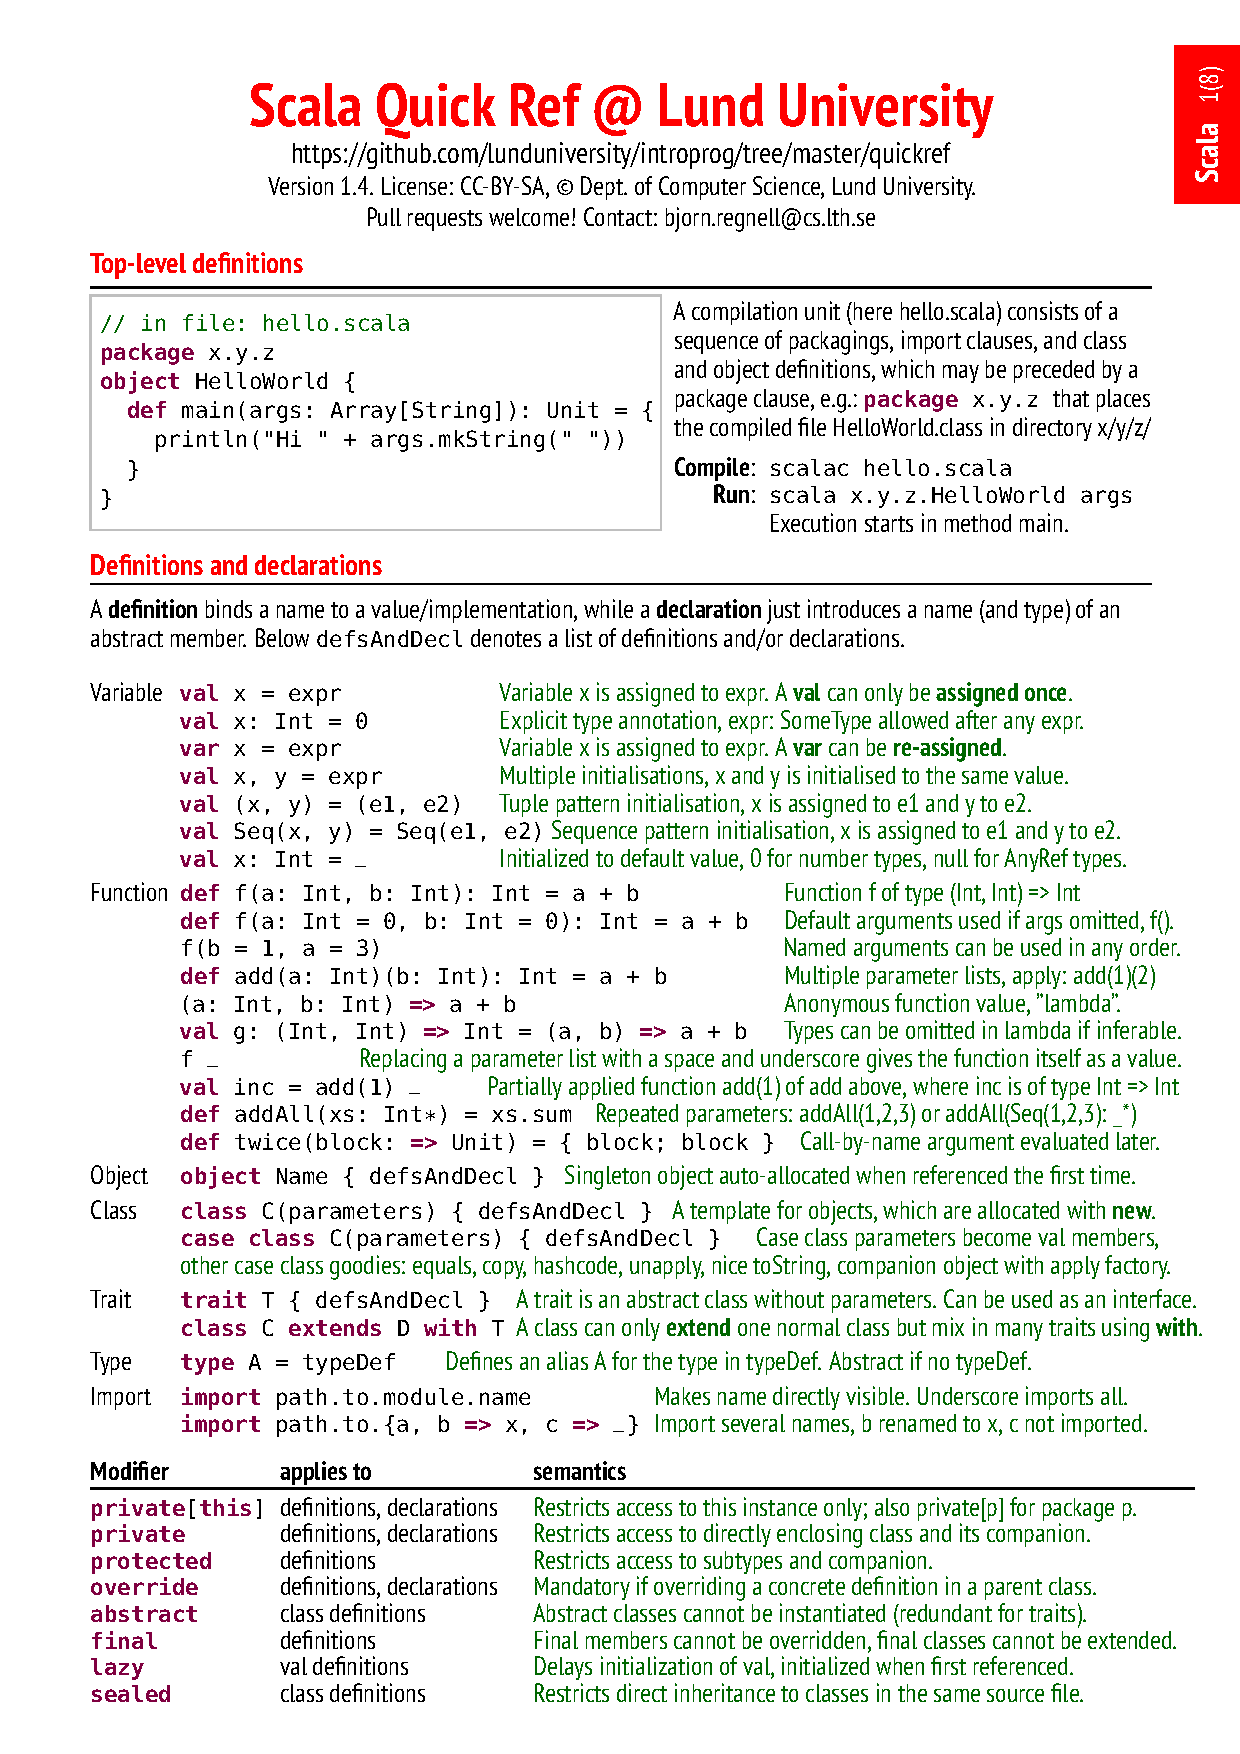
\includepdf[pages={1-12}, scale=0.77, frame]{../quickref/quickref.pdf}


\end{document}
